% This is samplepaper.tex, a sample chapter demonstrating the
% LLNCS macro package for Springer Computer Science proceedings;
% Version 2.20 of 2017/10/04
%
\documentclass[runningheads]{llncs}\usepackage[]{graphicx}\usepackage[]{color}
% maxwidth is the original width if it is less than linewidth
% otherwise use linewidth (to make sure the graphics do not exceed the margin)
\makeatletter
\def\maxwidth{ %
  \ifdim\Gin@nat@width>\linewidth
    \linewidth
  \else
    \Gin@nat@width
  \fi
}
\makeatother

\definecolor{fgcolor}{rgb}{0.345, 0.345, 0.345}
\newcommand{\hlnum}[1]{\textcolor[rgb]{0.686,0.059,0.569}{#1}}%
\newcommand{\hlstr}[1]{\textcolor[rgb]{0.192,0.494,0.8}{#1}}%
\newcommand{\hlcom}[1]{\textcolor[rgb]{0.678,0.584,0.686}{\textit{#1}}}%
\newcommand{\hlopt}[1]{\textcolor[rgb]{0,0,0}{#1}}%
\newcommand{\hlstd}[1]{\textcolor[rgb]{0.345,0.345,0.345}{#1}}%
\newcommand{\hlkwa}[1]{\textcolor[rgb]{0.161,0.373,0.58}{\textbf{#1}}}%
\newcommand{\hlkwb}[1]{\textcolor[rgb]{0.69,0.353,0.396}{#1}}%
\newcommand{\hlkwc}[1]{\textcolor[rgb]{0.333,0.667,0.333}{#1}}%
\newcommand{\hlkwd}[1]{\textcolor[rgb]{0.737,0.353,0.396}{\textbf{#1}}}%
\let\hlipl\hlkwb

\usepackage{framed}
\makeatletter
\newenvironment{kframe}{%
 \def\at@end@of@kframe{}%
 \ifinner\ifhmode%
  \def\at@end@of@kframe{\end{minipage}}%
  \begin{minipage}{\columnwidth}%
 \fi\fi%
 \def\FrameCommand##1{\hskip\@totalleftmargin \hskip-\fboxsep
 \colorbox{shadecolor}{##1}\hskip-\fboxsep
     % There is no \\@totalrightmargin, so:
     \hskip-\linewidth \hskip-\@totalleftmargin \hskip\columnwidth}%
 \MakeFramed {\advance\hsize-\width
   \@totalleftmargin\z@ \linewidth\hsize
   \@setminipage}}%
 {\par\unskip\endMakeFramed%
 \at@end@of@kframe}
\makeatother

\definecolor{shadecolor}{rgb}{.97, .97, .97}
\definecolor{messagecolor}{rgb}{0, 0, 0}
\definecolor{warningcolor}{rgb}{1, 0, 1}
\definecolor{errorcolor}{rgb}{1, 0, 0}
\newenvironment{knitrout}{}{} % an empty environment to be redefined in TeX

\usepackage{alltt}
% Insert the name of "your journal" with
% \journalname{myjournal}
%


%\let\origvec\vec
%\let\springervec\vec
%\let\vec\origvec
%\documentclass[smallextended]{svjour3}       % onecolumn (second format)
%\documentclass[twocolumn]{svjour3}          % twocolumn
%
%\smartqed  % flush right qed marks, e.g. at end of proof
%
\usepackage{amsmath,amssymb,array}
\usepackage{xcolor}
\usepackage{graphicx}
\usepackage{xargs}
\usepackage{sparklines}
% So that I can use the bars as interval visualizations
\setlength{\sparkspikewidth}{0.1mm}
\setlength{\sparklinethickness}{0.7pt}
\renewcommand{\sparklineheight}{2}
\usepackage[utf8]{inputenc}
%\usepackage[T1]{fontenc}
\usepackage{booktabs}
\usepackage{todonotes}
\usepackage[square,numbers,sort&compress,sectionbib]{natbib}
\renewcommand\citet{\cite}
\renewcommand{\bibname}{References}
% \usepackage[natbib=true]{biblatex}
% \bibliography{Bib}
\usepackage[hyphens]{url}
\usepackage{hyperref}
\renewcommand\UrlFont{\color{blue}\rmfamily}
\usepackage{colortbl}
\usepackage{csquotes} %[autostyle=true,german=quotes]
\usepackage{mathtools}
%\usepackage[section]{placeins} % forces figures within section
\usepackage{float} %https://tex.stackexchange.com/questions/165021/fixing-the-location-of-the-appearance-in-algorithmicx-environment
\usepackage{adjustbox}
%\usepackage{caption}[skip=2pt]
%\setlength{\abovecaptionskip}{5pt plus 0pt minus 2pt}
%\setlength{\belowcaptionskip}{5pt plus 0pt minus 2pt}
%\setlength{\intextsep}{10pt plus 2pt minus 2pt}
\usepackage{dsfont}
\usepackage[ruled, vlined, linesnumbered]{algorithm2e}
\DontPrintSemicolon                        % Don't print semicolon
\SetKwInput{KwInput}{Input}                % Set the Input
\SetKwInput{KwOutput}{Output}              % set the Output
\let\oldnl\nl% Store \nl in \oldnl
\newcommand{\nonl}{\renewcommand{\nl}{\let\nl\oldnl}}% Remove line number for one
\usepackage{cleveref}

\input{./latex-math/basic-ml.tex}
\input{./latex-math/basic-math.tex}

\newcounter{mycomment}
\newcommand{\mycomment}[2][]{%
    % initials of the author (optional) + note in the margin
    \refstepcounter{mycomment}%
    {%
    \todo[color={red!100!green!33},size=\small]{%
        \textbf{Comment [\uppercase{#1}\themycomment]:}~#2}%
    }}
\newcommand{\todoBH}[1]{\mycomment[BH]{#1}}


% Paper specific math
\newcommand{\xij}{x_{j}^{(i)}}                                         % i-th instance, j-th feature
%\newcommand{\fh}{f}
%  ALE decomposition
\newcommand{\fzero}{f_0}                                              % f_0 for ALE decomp
\newcommand{\falej}{f_{j,ALE}}                                        % ALE function for feature j
\newcommand{\faleme}{f_{ALE1st}}

% ALE approximation
\newcommand{\galej}{g_{j,ALE}^{\epsilon}}                               % Approximation of j-th ALE curve



\IfFileExists{upquote.sty}{\usepackage{upquote}}{}
\begin{document}

\title{Quantifying Model Complexity via Functional Decomposition for Better Post-Hoc Interpretability}
\titlerunning{Quantifying Model Complexity}

\author{
	Christoph Molnar %\orcidID{0000-0003-2331-868X}
	\and Giuseppe Casalicchio %\orcidID{0000-0001-5324-5966}
	\and Bernd Bischl %\orcidID{0000-0001-6002-6980}
}
\authorrunning{C. Molnar et al.}

\institute{Department of Statistics, LMU Munich, \\
  Ludwigstr. 33, 80539 Munich, Germany \\
  \email{christoph.molnar@stat.uni-muenchen.de}%\\
}

\maketitle

\begin{abstract}
Post-hoc model-agnostic interpretation methods such as partial dependence plots can be employed to interpret complex machine learning models.
%Both approaches have disadvantages.
While these interpretation methods can be applied regardless of model complexity, they can produce misleading and verbose results if the model is too complex, especially w.r.t. feature interactions.
%We propose to make the compromise between predictive power and interpretability explicit by quantifying the complexity / interpretability of machine learning models.
To quantify the complexity of arbitrary machine learning models, we propose model-agnostic complexity measures based on functional decomposition: number of features used, interaction strength and main effect complexity.
We show that post-hoc interpretation of models that minimize the three measures is more reliable and compact.
Furthermore, we demonstrate the application of these measures in a multi-objective optimization approach which simultaneously minimizes loss and complexity.
\keywords{Model Complexity \and Interpretable Machine Learning \and Explainable AI \and Accumulated Local Effects \and Multi-Objective Optimization}
\end{abstract}




\section{Introduction}
\label{sec:introduction}

%==============================================================================
% Interpretability requirement and trade-off
%==============================================================================
Machine learning models are optimized for predictive performance, but it is often required to understand models, e.g., to debug them, gain trust in the predictions, or satisfy regulatory requirements.
Many post-hoc interpretation methods either quantify effects of features on predictions, compute feature importances, or explain individual predictions, see \citep{molnar2019,guidotti2018survey} for more comprehensive overviews.
While model-agnostic post-hoc interpretation methods can be applied regardless of model complexity \citep{ribeiro2016model}, their reliability and compactness deteriorates when models use a high number of features, have strong feature interactions and complex feature main effects.
Therefore, model complexity and interpretability are deeply intertwined and reducing complexity can help to make model interpretation more reliable and compact.
% =============================================================================
% Need interpretability measures
% =============================================================================
Model-agnostic complexity measures are needed to strike a balance between interpretability and predictive performance \citep{ruping2006learning,bibal2016interpretability}.

% =============================================================================
% Our solution
% =============================================================================
\textbf{Contributions.}
We propose and implement three model-agnostic measures of machine learning model complexity which are related to post-hoc interpretability.
To our best knowledge, these are the first model-agnostic measures that describe the global interaction strength, complexity of main effects and number of features.
%For the \textbf{number of features used} by the model, we propose an estimation heuristic.
%Based on the decomposition of the prediction function, we suggest measures for \textbf{interaction strength} and for \textbf{average complexity of the feature main effects}.
We apply the measures to different datasets and machine learning models.
We argue that minimizing these three measures improves the reliability and compactness of post-hoc interpretation methods.
Finally, we illustrate the use of our proposed measures in multi-objective optimization.




\section{Related Work and Background}
\label{sec:related}

In this section, we introduce the notation, review related work, and describe the functional decomposition on which we base the proposed complexity measures.

\textbf{Notation:} We consider machine learning prediction functions $f:\mathbb{R}^p \mapsto \mathbb{R}$, where $f(x)$ is a prediction (e.g., regression output or a classification score).
For the decomposition of $f$, we write $f_S:\mathbb{R}^{|S|} \mapsto \mathbb{R}$, $S \subseteq\{1, \ldots, p\}$, to denote a function that maps a vector $x_S \in \mathbb{R}^{|S|}$ with a subset of features to a marginal prediction.
If subset $S$ contains a single feature $j$, we write $f_j$.
We refer to the training data of the machine learning model with the tuples $\D = \{(x^{(i)},y^{(i)})\}_{i=1}^n$ and refer to the value of the $j$-th feature from the $i$-th instance as $x_j^{(i)}$.
We write $X_j$ to refer to the $j$-th feature as a random variable.

\textbf{Complexity and Interpretability Measures:}
\label{sec:other}
% =============================================================================
% Model-specific or class-specific measures of interpretability
% =============================================================================
In the literature, model complexity and (lack of) model interpretability are often equated.
Many complexity measures are model-specific, i.e., only models of the same class can be compared (e.g., decision trees).
Model size is often used as a measure for interpretability (e.g., number of decision rules, tree depth, number of non-zero coefficients) \citep{huysmans2011empirical,ruping2006learning,askira1998knowledge,yang2017scalable,schielzeth2010simple,lakkaraju2017interpretable,furnkranz2012foundations,ustun2016supersparse}.
Akaikes Information Criterion (AIC) %\citep{akaike1998information}
and the Bayesian Information Criterion (BIC)
%\citep{schwarz1978estimating}
are more widely applicable measures for the trade-off between goodness of fit and degrees of freedom.
%AIC and BIC fix a certain compromise between interpretability and performance, and consider only one dimension of interpretability, the degrees of freedom.
% =============================================================================
% Model-agnostic measures
% =============================================================================
In \citep{philipp2018measuring}, the authors propose model-agnostic measures of model stability.
In \citep{plumb2019regularizing}, the authors propose explanation fidelity and stability of local explanation models.
% =============================================================================
% Other approaches
% =============================================================================
Further approaches measure interpretability based on experimental studies with humans, e.g., whether humans can predict the outcome of the model \citep{zhou2018measuring,huysmans2011empirical,dhurandhar2017tip,poursabzi2018manipulating,friedler2019assessing}.

\textbf{Functional Decomposition:}
\label{sec:decomposition}
% =============================================================================
% General decomposition
% =============================================================================
Any high-dimensional prediction function can be decomposed into a sum of components with increasing dimensionality:

\begin{eqnarray}\label{eqn:decomp} f(x)  = &\overbrace{f_0}^\text{Intercept} + \overbrace{\sum_{j=1}^p f_j(x_j)}^\text{1st order effects} + \overbrace{\sum_{j<k}^p f_{jk}(x_j, x_k)}^\text{2nd order effects} + \ldots + \overbrace{f_{1,\ldots,p}(x_1, \ldots, x_p)}^\text{p-th order effect}
%\\ =  & \sum_{S \subseteq \{1,\ldots,p\}} f_S(x_S)
\end{eqnarray}
% =============================================================================
% Some useful decompositions
% =============================================================================
This decomposition is only unique with additional constraints regarding the components.
%For example, you can set all components to 0, and define the last component as the difference between the arbitrary decomposition and the true model function.
%Stone \citep{stone1994use} suggested orthogonality constraints and approximating the prediction function with weighted integrals.
%Hooker \citep{hooker2007generalized} defined centering, orthogonality and variance decomposition as desirable properties, resulting in unique and hierarchically orthogonal components under the correlation inner product.
% =============================================================================
% ALE decompositions
% =============================================================================
Accumulated Local Effects (ALE) were proposed in \cite{apley2016visualizing} as a tool for visualizing feature effects (e.g., Figure~\ref{fig:c-demo}) and as unique decomposition of the prediction function with components $f_S = f_{S,ALE}$.
The ALE decomposition is unique under an orthogonality-like property described in \citep{apley2016visualizing}.

%\begin{eqnarray}
%f(x)  = & f_0 + \sum_{j=1}^p \falej(x_j)+ \sum_{j\neq k}^p f_{ALE,jk}(x_j, x_k) + \ldots + f_{ALE,1,\ldots,p}(x_1, \ldots, x_p)
%\end{eqnarray}
% =============================================================================
% ALE definition
% =============================================================================

The ALE main effect $f_{j,ALE}$ of a feature $x_j, j \in \{1,\ldots,p\}$ for a prediction function $f$ is defined as
\begin{eqnarray}\label{eqn:ale}
\falej(x_j) = \int_{z_{0,j}}^{x_j} \mathbb{E}\left[\frac{\partial f(X_1,\ldots,X_p)}{\partial X_j}\middle|X_j = z_j\right]dz_j-c_j
\end{eqnarray}
Here, $z_{0,j}$ is a lower bound of $X_j$ (usually the minimum of $x_j$) and the expectation $\mathbb{E}$ is computed conditional on the value for $x_j$ and over the marginal distribution of all other features.
The constant $c_j$ is chosen so that the mean of $f_{j,ALE}(x_j)$ with respect to the marginal distribution of $X_j$ is zero, so that the ALE components sum to the full prediction function.
By integrating the expected derivative of $f$ with respect to $X_j$ the effect of $x_j$ on the prediction function $f$ is isolated from the effects of all other features.
ALE main effects are estimated with finite differences, i.e., access to the gradient of a prediction function is not required (see \citep{apley2016visualizing}).
% =============================================================================
% ALE is best
% =============================================================================
We base our proposed measures on the ALE decomposition, because ALE are computationally cheap (worst case $O(n)$ per main effect), they can be computed sequentially instead of simultaneously, they do not require knowledge of the joint distribution, and several software implementations exist \citep{iml,alepackage}.

% =============================================================================
% =============================================================================
% =============================================================================
% Material
% =============================================================================
% =============================================================================
% =============================================================================
% Categorical features
%Categorical features require an ordering of the categories so that accumulated local effects can be estimated.
%Any ordering of the categories will yield a valid ALE, but the interpretation differs, because category effects are interpreted in terms of changes to the neighbouring categories.
%Compared to \citep{hooker2007generalized}, ALE yields a fundamentally different decomposition of the model function $f(x)$.
%\citep{apley2016visualizing} show that this decomposition is unique because of what they call "pseudo-orthogonality".
%Pseudo-orthogonality means that for any component of the ALE decomposition, a repeated application of ALE computation yields zero or the same ALE component (if the same ALE effect is computed).
%For example, lets look at the 1st-order (=main) effect of $x_1$ $f_{ALE,1}$ and the second order effect between $x_1$ and $x_2$ $f_{ALE,1,2}$.
%If we tried to extract the main order effect for $x_1$ from $f_{ALE, 1,2}$ the result would be a constant function that is always 0.
% =============================================================================
% ALE property: Pseudo-orthogonality
% =============================================================================
%Let $H_S(f_S)$ be a function that maps a function to its ALE function with features S.
%ALE defines the components in such a way that they are "pseudo-orthogonal", which is not true orthogonality, but a similar concept.
%"Pseudo-orthogonality": $H_j(f_j) = f_j$ and $H_u(f_j) = 0$ for each $j \subseteq D$ and $u \subseteq D$ with $u \neq j$.
%In words, pseudo-orthogonality is:
%The S-ALE of an S-ALE function is again S-ALE and the S-ALE function of u-ALE is 0 when S and u are not equal.

%We prefer the orthogonality-like  over orthogonality, since when feature are correlated, the true additive structure is not reflected when effects have to be orthogonal.
%%For example if the model is a linear model with $f(x) = x_1 + 2\cdot x_2$, with $x_1$ and $x_2$ being correlated, we prefer to recover $f_{1}(x_1) = 1$ and $f_{2}(x_2)$ which is the result under ALE decomposition, but not under the constraint of orthogonality.

% =============================================================================
% Concepts for interpretability
% =============================================================================
%There are a few concepts of interpretability.
%Other suggested measures of interpretability is to constrain model form:
%Monotonicity constraints: CITE.
%Causality.CITE.
%Additivity. CITE.
%Sparsity. CITE.
%Linearity. CITE.





% =============================================================================
% Some taxonomy
% =============================================================================
% \citep{bibal2016interpretability} distinguish between interprebaility on model level and on representation level.
% This adds to the taxonomy of \citep{doshi2017towards}
% Quantiative measurements of model: Either some heuristic of model (e.g. number of features in Lasso) or user-based surveys \citep{freitas2014comprehensible}.
% Quantiative heuristic measure model.
% User-based surveys measure representation

% =============================================================================
% Categorization of our method
% =============================================================================
% According to \citep{bibal2016interpretability} we can distinguish measures of interpretability for following areas.
% \begin{itemize}
% \item model (specific, general)
% \item representation (specific, general)
% \end{itemize}
% Our method depends on representation and on the model of course.
% So something in between.



% Pseudo-orthogonality > Orthogonality
% True orthogonality is not desirable, as illustrated with this next example.
% For example if $f(x) = x_1 + x_2$ and $X_1$ and $X_2$ are correlated, then fANOVA decomposition will not give the correct main effects $f_1(x_1)$ and $f_2(x_2)$, but ALE components will decompose it in such a way.
% For fANOVA approach this would be.
% We assume that expected value of $x_1$ and $x_2$ is 0:
% \begin{eqnarray*}
% f_{1,fANOVA}(x_1) =& \mathbb{E}(f(x)|X_1=x_1) - E_X(f(x)) \\
%                   =& \mathbb{E}(X_1| X_1=x_1) + \mathbb{E}(X_2|X_1 = x_1) - (\mathbb{E}(X_1) + \mathbb{E}(X_2)) \\
%                   =& x_1 +  \mathbb{E}(X_2|X_1 = x_1)  \\
%                   \neq & x_1
% \end{eqnarray*}
% Intuition: Feature x1 and x2 are correlated. But effects are forced to be non-correlated.



\section{Functional Complexity}
\label{sec:measures}

% =============================================================================
% General idea in words
% =============================================================================
In this section, we motivate complexity measures based on functional decomposition.
% =============================================================================
% Decomposition and Simplification
% ============================================================================
Based on Equation~\ref{eqn:decomp}, we decompose the prediction function into a constant (estimated as $f_0 = \frac{1}{n}\sum_{i=1}^n f(\xi)$), main effects (estimated by ALE), and a remainder term containing interactions (i.e., the difference between the full model and constant + main effects).

\begin{eqnarray} f(x) % = &\overbrace{f_0}^\text{Intercept} + \overbrace{\sum_{j=1}^p f_j(x_j)}^\text{1st order effects} + \overbrace{\sum_{S \subseteq \{1,\ldots,p\},|S| \geq 2} f_{S}(x_S)}^{\text{Higher order effects}} \\
=&\underbrace{f_0 + \sum_{j=1}^p \overbrace{\falej(x_j)}^\text{MEC: How complex?} + \overbrace{IA(x)}^{\text{IAS: Interaction strength?}}}_{\text{NF: How many features were used?}}
\end{eqnarray}
This arrangement of components emphasizes a decomposition of the prediction function into a main effect model and an interaction remainder.
We can analyze how well the main effect model itself approximates $f$ by looking at the magnitude of the interaction measure IAS.
The average main effect complexity (MEC) captures how many parameters are needed to describe the one-dimensional main effects on average.
The number of features used (NF) describes how many features were used in the full prediction function.
% =============================================================================
% Why minimize proposed measures?
% =============================================================================
%When the three measures are minimized, the following improvements of interpretability will be reached.
%Minimizing the number of features to be used directly improves the sparsity of the model.
%The less features are used, the less plots have to be looked at and the less numbers are needed to describe e.g. the feature importance and so on.
%Minimizing the strength of interactions increases how much of the prediction variance the main effects explain.
%If the interaction measure is zero, the ALE plots will explain all of the models variance.
%Minimizing the complexity of the first order effects ensures that we need less parameters to (approximately) describe the main effects.
%A complexity of 1 means that we only need a single number to describe the relationship.




% -----------------------------------------------------------------------------
% Material
% -----------------------------------------------------------------------------
%These measures quantify the complexity of a machine learning model from an external view onto the shape of the prediction function and ignores the actual representation of the model (e.g. tree structure).


% We do the following approximation:
%
% \begin{eqnarray*}
% f(x)  =& \overbrace{f_0}^\text{Intercept} + \overbrace{\sum_{j=1}^p f_j(x_j)}^\text{1st order effects} + \overbrace{\sum_{j\neq k}^p f_{jk}(x_{jk})}^\text{2nd order effects} + \ldots + \overbrace{f_{1,\ldots,p}(x_{1,\ldots,p})}^\text{p-th order effect}\\
%      =& f_0 + \sum_{j=1}^{p} f_{j}(x_j) + \sum_{S \subseteq \{1,\ldots,p\}} f_{S}(x_S)\\
%      =& \bar{f}(x) + \sum_{j=1}^{p} f_{j,ALE}(x_j)  + IA(x) \\
%      =& \bar{f}(x) + \sum_{j=1}^{p} (\tilde{f}_{j,ALE}(x_j) + \epsilon_{j}(x_j)) + IA(x) \\
% \end{eqnarray*}
%
% $\tilde{f}_{j,ALE}(x_j) $ is the approximation of the j-th main effect.\\
% $\epsilon_{j}(x_j)$ is the approximiation error $f_{j,ALE}(x_j) - \tilde{f}_{j,ALE}(x_j)$\\
% $IA(x)$ the interaction terms.\\


% \citep{murdoch2019interpretable} defines the following desiderata for an interpretability measure:
% Accuracy
% \begin{itemize}
% \item Accuracy (of interpretation method), which matches that we look at R squared. Predictive accuracy is measured as usual. Descriptive accuracy is measured with novel measures
% \item Relevancy: Show only relevant information. With our measures we can decide which plots to show. Remove when effect is zero. Also we can measure variance of each of the 1st order components and only show the most relevant ones.
% \item Sparsity: Directly optimized with our measures
% \item Simulatability: Can human internally simulate and reason about
% \item Modularity: Can model parts be interpreted independently? Interaction measure allows us to determine how independently we can analyze the individual features with their ALE plots
% \item They also say: "Moreover, it is unclear if any of the current interpretation forms can fully capture a model’s behaviour, or if a new format altogether is needed. How to close that gap, while producing outputs relevant to a particular audience/problem, is an open problem."
% \end{itemize}
%
% We claim that optimizing the two measures we will propose will improve those desiderata:
% Decreasing interactions will improve the accuracy of the view of ALE first order plots.
% modularity is achieved by doing a decomposition.
% With interaction measure you can see how much the first order ALE plots of the variance already explain.





\subsection{Number of Features (NF)}
\label{sec:nfeatures}

% =============================================================================
% About sparsity
% =============================================================================
We propose an approach based on feature permutation to determine how many features are used by a model.
We regard features as "used" when changing a feature changes the prediction.
If available, the model-specific number of features is preferable.
The model-agnostic version is useful when the prediction function is only accessible via API or when the machine learning pipeline is complex.

% =============================================================================
% Why model-agnostic
% =============================================================================\
%f available, a model-specific method for extracting the number of features used by the model is preferable, e.g. counting the number of non-zero weights in a sparse linear regression model.
% model-agnostic heuristic is useful when the prediction function is accessible but not the internal structure of the model (e.g. prediction via API call), or when combining preprocessing steps and models complicates programmatic extraction (e.g. training a decision tree on sparse principal components).

% =============================================================================
% Feature-count heuristic: intuition
% =============================================================================
The proposed procedure is formally described in Algorithm~\ref{algo:nfeat}.
To estimate whether the $j$-th feature was used, we sample instances from data $\D$, replace their $j$-th feature values with random values from the distribution of $X_j$ (e.g., by sampling $\xj$ from other instances from $\D$), and observe whether the predictions change.
If the prediction of any sample changes, the feature was used. 
% =============================================================================
% Feature-count heuristic: algorithm
% =============================================================================
\begin{algorithm}
\caption{Number of Features Used (NF)}\label{algo:nfeat}
\KwInput{Number of samples $M$, data $\D$}
NF = 0\;
	\For{$j \in 1,\ldots,p$}{
		Draw $M$ instances $\{x^{(m)}\}_{m=1}^M$ from dataset $\D$\;
			Create $\{x^{(m)*}\}_{m=1}^M$ as a copy of $\{x^{(m)}\}_{m=1}^M$ \;
			\For{$m\in 1,\ldots,M$}{
				Sample $\xj^{(new)}$ from $\{\xij\}_{i=1}^n$ with the constraint that $\xj^{(new)} \neq \xj^{(m)}$\;
				Set $\xj^{(m)*} = \xj^{(new)}$\;
			}
			\lIf{$\fh(x^{(m)*}) \neq \fh(x^{(m)}) \text{ for any }  m \in \{1,\ldots,M\}$}{$NF = NF + 1$.
		}
		}
\Return NF
\end{algorithm}
%
% =============================================================================
% False negatives
% =============================================================================
%The rate of false positives is zero, i.e. the probability that the heuristic counts a feature as used, but the model did not use the feature is zero.
%The probability of a false negative, i.e. the heuristic overlooks a feature, depends on the number of samples $M$, the model function $f$ and the data distribution.
%Let $P_{dep}^j$ be the probability that the prediction of a random instance depends on the value of $x_j$.
%For an instance that depends on $x_j$ for its prediction, let $P_{change}^j$ be the probability that a sample from $X_j$ changes the prediction for an instance i.
%Then the probability of overlooking feature j is: $P_{fn}^j=(1 - P_{dep}^j + P_{dep}^j (1 - P_{change}^j))^M$
%With the simplifying assumption that $P_{fn}^j = P_{fn} \forall j \in 1,\ldots,p$, the probability that we miss at least one feature is $1 - (1 - P_{fn})^p$.
%For a linear model without interactions and only numerical features, the false negative rate is 0:
%$P_{dep}^j=1$ and $P_{change}^j = 1$, so that $P_{fn}^j = (1 - 1 + 0)^M = 0$.
%Let us assume a non-linear model where only one percent of instances rely on feature $\xj$ ($P_{dep}^j=0.01$) and these instances have a probability of 0.02 that the feature permutation changes the prediction ($P_{change}^j=0.02$).
%If we set $M=100$, then $P_{fn}^j = (0.99 + 0.01\cdot 0.01)^{100} \approx 0.37$.
%If we increase M to 500, the probability that NF counts too few features drops to $\approx 0.007$.



We tested the NF heuristic with the Boston Housing data.
We trained decision trees (CART) with maximum depths $\in\{1,2,10\}$ leading to 1, 2 and  4 features used and an L1-regularized linear model with penalty $\lambda\in\{10, 5, 2, 1, 0.1, 0.001\}$ leading to 0, 2, 3, 4, 11 and 13 features used.
For each model, we estimated NF with sample sizes $M\in\{10, 50, 500\}$ and repeated each estimation 100 times.
For the elastic net models, NF was always equal to the number of non-zero weights. 
For CART, the mean absolute differences between NF and number of features used in the trees were 0.300 ($M=10$), 0.020 ($M=50$) and 0.000 ($M=500$).




\subsection{Interaction Strength (IAS)}
\label{sec:interaction}


% =============================================================================
% First order model
% =============================================================================
Interactions between features mean that the prediction cannot be expressed as a sum of independent feature effects, but the effect of a feature depends on values of other features \citep{molnar2019}.
We propose to measure interaction strength as the scaled approximation error between the ALE main effect model and the prediction function $f$.
Based on the ALE decomposition, the ALE main effect model is defined as the sum of first order ALE effects:
$$\faleme(x) = f_0 + f_{1,ALE}(x_1) + \ldots + f_{p,ALE}(x_p)$$
% =============================================================================
% PRE / PRL
% =============================================================================
We define interaction strength as the approximation error measured with loss $L$:
\begin{eqnarray}\label{eqn:pre}
IAS = \frac{\mathbb{E}(L(f, \faleme))}{\mathbb{E}(L(f, f_0))} \geq 0
\end{eqnarray}
Here, $f_0$ is the mean of the predictions and can be interpreted as the functional decomposition where all feature effects are set to zero.
% =============================================================================
% R2 special case
% =============================================================================
IAS with the $L2$ loss equals 1 minus the R-squared measure, where the true targets $y_i$ are replaced with $f(\xi)$.
$$IAS = \frac{\sum_{i=1}^n(f(\xi)-\faleme(\xi))^2}{\sum_{i=1}^n(f(\xi) - f_0)^2} = 1 - R^2$$
% Interpretation of IAS
% =============================================================================
If $IAS=0$, then $L(f,\faleme)=0$, which means that the first order ALE model perfectly approximates $f$ and the model has no interactions.
%IAS can be larger than $0$ for additive models for which we would expect $IAS=0$, as observed in e.g. Table~\ref{tab:pareto} (e.g. $IAS=0.01$).
%This small deviation can occur when the true ALEs (see Equation~\ref{eqn:ale}) are not perfectly approximated by finite differences.
% =============================================================================
% =============================================================================
% Further Material
% =============================================================================
% =============================================================================

% =============================================================================
% Further approaches
% =============================================================================
%There are other ways to estimate the additivity of a model.
%One is via Sobol interaction strength \citep{sobol1993sensitivity} or Shapley \citep{owen2014sobol}.
%We decided against Sobol and Shapley since they were computationally expensive and varied a lot from run to run.
%Additionally it makes more sense to look at the PRL/PRE of the main effects of the decomposition, since then it is coherent with the plots that are shown and with the complexity, which is presented next.




% =============================================================================
% pre algorithm
% =============================================================================
%The estimation of the pre of the main effects ALE model is described with the following algorithm.
%\begin{algorithm}
%\caption{Estimate PRL of ALE main effects model}\label{algo:ale1st}
%\begin{enumerate}
%\item Given: model $f$, dataset $\D$, loss function $L$
%\item Estimate $\falej$ for all features $j\in\{1,\ldots,p\}$
%\item Estimate $\fzero = \sum_{i=1}^n f(\xi)$
%\item Define: $\fale(x) = \fzero + \sum_{j=1}^p \falej(x)$
%\item Calculate $PRL(L, f, \fale)$
%\end{enumerate}
%\end{algorithm}






\subsection{Main Effect Complexity (MEC)}
\label{sec:curve}

% =============================================================================
% Measure Intro
% =============================================================================

To determine the average shape complexity of ALE main effects $\falej$, we propose the main effect complexity (MEC) measure.
For a single ALE main effect, we define $\text{MEC}_j$ as the number of parameters needed to approximate the curve with piece-wise linear models.
For the entire model, MEC is the average $\text{MEC}_j$ over all main effects, weighted with their variance.
Figure~\ref{fig:c-demo} shows an ALE plot (= main effect) and its approximation with two linear segments.
%

%

%
%

%
%
\begin{knitrout}\small
\definecolor{shadecolor}{rgb}{0.969, 0.969, 0.969}\color{fgcolor}\begin{figure}

{\centering 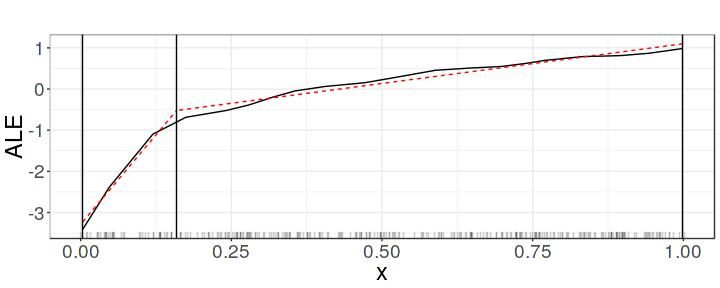
\includegraphics[width=10cm,height=4cm]{knit-fig/c-demo-1} 

}

\caption[ALE curve (solid line) approximated by two linear segments (dotted line)]{ALE curve (solid line) approximated by two linear segments (dotted line).}\label{fig:c-demo}
\end{figure}


\end{knitrout}
% =============================================================================
% Measure Intuition
% =============================================================================
We use piece-wise linear regression to approximate the ALE curve.
Within the segments, linear models are estimated with ordinary least squares.
The breakpoints that define the segments are found by greedy and exhaustive search along the interval boundaries of the ALE curve.
Greedy here means that we first optimize the first breakpoint, then the second breakpoint with the first breakpoint fixed and so on.
We measure the degrees of freedom as the number of non-zero coefficients for intercepts and slopes of the linear models.
The approximation allows some error, e.g., an almost linear main effect may have $\text{MEC}_j=1$, even if dozens of parameters would be needed to describe it perfectly. 
The approximation quality is measured with R-squared ($R^2$), i.e., the proportion of variance of $\falej$ that is explained by the approximation with linear segments.
An approximation has to reach an $R^2 \geq 1-\epsilon$, where $\epsilon$ is the user defined maximum approximation error.
We also introduced parameter $max_{seg}$, the maximum number of segments.
In the case that an approximation cannot reach an $R^2 \geq 1-\epsilon$ with a given $max_{seg}$, $\text{MEC}_j$ is computed with the maximum number of segments.
The selected maximum approximation error $\epsilon$ should be small, but not too small.
We found $\epsilon$ between $0.01$ and $0.1$ visually meaningful (i.e. a subjectively good approximation) and used $\epsilon=0.05$ throughout the paper.
We apply a post-processing step that greedily sets slopes of the linear segments to zero, as long as $R^2\in\{1-\epsilon,1\}$.
The post-processing potentially decreases the $\text{MEC}_j$, especially for models with constant segments like decision trees.
% =============================================================================
% Measure Sum Up and Fix
% =============================================================================
$\text{MEC}_j$ is averaged over all features to obtain the global main effect complexity.
Each $\text{MEC}_j$ is weighted with the variance of the corresponding ALE main effect to give more weight to features that contribute more to the prediction.
%For example, the two ALE curves  spark(app1_wiggle$ale, c(-7, 7), width = 5) and spark(app2_jump$ale, c(-7, 7), width = 5) are identical except for the jump at 0.5 in the second curve.
%We need more linear segments to get the same approximation $R^2$ as for the second curve.
%One way to mitigate the problem of getting high MEC estimates through wiggly main effects that are irrelevant for the prediction is to weight each main effect by its variance.
%For example, the  main effect curves spark(app1$ale, c(-6, 6), width = 5), spark(app2$ale, c(-6, 6), width = 5) and spark(app3$ale, c(-6, 6), width = 5) differ from each other by a scaling factor in the y-axis, but each requires five segments to be approximated with $R^2 >= 0.95$:
% spark(app1, c(-6, 6), width = 5), spark(app2, c(-6, 6), width = 5), and spark(app3, c(-6, 6), width = 5).
%When weighted with the variance,  spark(app1$ale, c(-6, 6), width = 5) gets a weight of sprintf("%.2f", app1$var), spark(app2$ale, c(-6, 6), width = 5) a weight of sprintf("%.2f", app2$var) and spark(app3$ale, c(-6, 6), width = 5) a weight of sprintf("%.2f", app3$var).
Algorithm~\ref{algo:AMEC} describes the MEC computation in detail.

% =============================================================================
% Algorithm for complexity
% =============================================================================
\begin{algorithm}
\caption{Main Effect Complexity (MEC).}\label{algo:AMEC}
	\KwInput{Model $f$, approximation error $\epsilon$, max. segments $max_{seg}$, data $\D$}
	Define $R^2(g_j, \falej) := \sum_{i=1}^n (g_j(\xij) - \falej(\xij))^2 / \sum_{i=1}^n (\falej(\xij))^2$\;
	\For{$j \in \pset$}{
        Estimate $\falej$\;
	\tcp{Approximate ALE with linear model}
	Fit $g_j(x_j) = \beta_0 + \beta_1 x_j$ predicting $\falej(\xij)$ from $\xij$, $i\in{1,\ldots,n}$\;
	Set $K=1$\;
	\tcp{Increase nr. of segments until approximation is good enough}
	\While{$K < max_{seg}$ AND $R^2(g_j,\falej) < (1- \epsilon)$}{
	        \tcp{Find intervals $Z_k$ through exhaustive search along ALE curve breakpoints}
		\tcp{For categorical feature, set slopes $\beta_{1,k}$ to zero}
		$g_j(x_j) = \sum_{k=1}^{K+1} \I_{\xj\in Z_k}\cdot\left(\beta_{0,k} + \beta_{1,k}\xj\right)$\;
		Set $K = K+1$
	}
	Greedily set slopes to zero while $R^2>1-\epsilon$\;
	%\tcp{Post-processing of slopes}
	%\For{$k \in 1,\ldots,K$}{
	%	\tcp{$n_k$ is number of instances in interval $Z_k$}
	%	Set $\beta_{0,k} = \frac{1}{n_k}\sum_{i:\xi\in Z_k}\cdot\falej(\xij)$ and $\beta_{1,k} = 0$ in $g_j$\;
	%	\lIf{$R^2(g_j, \falej) > (1-\epsilon)$}
	%	{
	%		Use new $\beta_{0,k}$, $\beta_{1,k}$ in $g_j$
	%	}
	%	\lElse{
	%		Keep old $\beta_{0,k}$, $\beta_{1,k}$ in $g_j$
	%		}
	%		}
\tcp{Sum of non-zero coefficients minus first intercept}
	$MEC_j = K + \sum_{k=1}^K \mathbb{I}_{\beta_{1,k} > 0} - 1$\;
$V_j = \frac{1}{n}\sum_{i=1}^n (\falej(x^{(i)}))^2$\;
}
	\Return{$MEC = \frac{1}{\sum_{j=1}^pV_j}\sum_{j=1}^p V_j \cdot MEC_j$\;}
\end{algorithm}



% =============================================================================
% Experiment
% =============================================================================


%We tested the extraction of linear segments with a model for which we can validate if the correct segments were extracted: Multivariate Adaptive Regression Splines (MARS).
%In our experiment, we used the Boston housing data, trained a MARS model, extracted MEC and compared the slopes estimated by MARS and the ones estimated by our ALE approximation which is computed for the MEC.
%For each datapoint and each feature, we computed both the slopes for MARS and ALE approximation, and compared both using the cosine similarity.
%We see the lines at a data point as equivalent if cosine distance $\in\{0.999,1\}$.


% =============================================================================
% =============================================================================
% =============================================================================
% Material
% =============================================================================
% =============================================================================
% =============================================================================

% =============================================================================
% AMEC ignores internal model complexity and uses external complexity
% =============================================================================




%If all features in the data are uncorrelated, this has the nice interpretation that each feature main effect complexity (MEC) is weighted by the percentage it contributed to the variance of the complete main effects model.
%In case of correlated features, it's more complicated.
%If we were to fairly assign to each feature the share of the first order model variance, we would need an attribution method such as the Shapley value.
%The big problem is that the contribution can be negative when features are correlated and one of the correlated features has a much stronger effect.
%This can happen when the covariance is negative.
%The interpretation is not very intuitive then.
%An advantage of weighting by the individual variances is that it has a visual connection:
%The smaller the variance, the lower the amplitude of the curve in y-direction.
%And we want that weighted by the data distribution, so taking the minimum and maximu for scaling is not an option.


% =============================================================================
% Find best splits
% =============================================================================
%\begin{algorithm}
%\caption{ApproxLinearSegments}\label{algo:aleapprox}
%	\KwInput{K, $\falej$, $\epsilon$}
%	\KwOutput{$\beta \in \mathbb{R}^k, R^2$}
%	Define equidistant initial breakpoints: $\hat{z}_1,\ldots, \hat{z}_K$\;
%	Define segments $Z_1 = [min(\xj), z_1], \ldots, Z_k = [z_{k-1}, z_k],\ldots,Z_{K+1} = [z_K,max(\xj)]$ \\
%If $K=0$, then $Z_1 = [min(\xj), max(\xj)]$\;
%
%	Optimize break points: $\hat{z}_1,\ldots, \hat{z}_K = argmin_{z_1,\ldots,z_K} \sum_{k=1}^{K+1} \sum_{\xi\in Z_k}\left(\falej(\xij) - (\beta_{j0}^k + \beta_{j1}^k\xij)\right)^2$ where and $\beta_{j0}^k$ and $\beta_{j1}^k$ are the least square estimates.
%Optimize with Generalized Simulated annealing.
%
%$\galej(\xj) = \sum_{k=1}^{K+1} \I_{\xi\in Z_k}\left(\hat{\beta}_0^k + \hat{\beta}_j^k\xij\right)$.
%Set slopes to zero. For each segment $k \in 1,\ldots,K$:
%\begin{itemize}
%\item Set $\beta_{j0}^k = \frac{1}{n_k}\sum_{\xi\in Z_k}\falej(\xij)$ and $\beta_{j1}^k$ = 0
%\item If still $R^2 > 1 - \epsilon$, overwrite both $\beta$.
%\end{itemize}
%
%* If the feature is numeric, fix all $\beta_{j1}^k$ at zero and we applied random search of break points instead of GenSA.
%\end{algorithm}


% =============================================================================
% C example
% =============================================================================
% We illustrate the measure with a short example.
% We simulated 500 data points with 4 features as a regression problem \citep{friedman1991multivariate}.
% The features are uniformly distributed in the following intervals: $0\leq x_1 \leq 100$, $ 40\pi \leq x_2 \leq 560 \pi$, $ 0 \leq x_3 \leq 1$, $ 1 \leq x_4 \leq 11$.
% The regression target was simulated as:
%
% $$y = (x_1^2 + (x_2 \cdot x_3 - (1/(x_2 \cdot x_4)))^2)^{0.5} + e$$
% where $ e \sim N(0,125)$.
%
% We trained a random forest, plotted the ALEs and calculated the complexities with the parameters $\epsilon = 0.95$, $max_{segnum} = 5$ and $max_{segcat} = 9$


% Since the model relied the most on $x2$ and $x3$ as main effects, the weighted main effect complexity is fc$c_wmean.
% Both features main effects can be approximated with a linear segment.
% The other two feature have a very low variance and get a low weight.


% =============================================================================
% Different epsilons
% =============================================================================
%The choice of $\epsilon$ affects the complexity measures:
%This ALE main effect spark(fc1$approx_models$V3$ale) can be approximated with a linear model spark(fc1$approx_models$V3, approx = TRUE) when $\epsilon = eps1$ but needs (fc3$approx_models$V3$n_coefs + 1) / 2 segments when $\epsilon$ is decreased to eps3: spark(fc3$approx_models$V3, approx = TRUE).



% =============================================================================
% Did not work out
% =============================================================================
% We tried a few alternatives to approximate the ALE plots for measuring their complexity, which turned out to be impractical.
% We tried approximation with cubic (overlapping) splines and measuring the complexity as degrees of freedom.
% The degrees of freedom exploded when the ALE plot was not quite linear, but almost, yielding an unintuitive measure.
% Tree splits did not work, like for example model based partitioning TODO: CITE mob.
% One reason is that the greedy approach did not work well and we found it better to search per number of splits.

%The complexity measures ignores how complex the internal structure of the model is, e.g. it does not matter whether the linear relationship comes from a single linear model or a blend of hundreds of linear models.
%We demonstrate how the number of nodes and complexity measure C increase with increasing model performacne, but at some point the complexity C decreases again.
%For this example, n data points were drawn from a uniform distribution between 0 and 1, and the target is simulated as $2 * x + \epsilon$, where $\epsilon \sim N(0,nsd)$.
%We trained three trees with different maximal depths, as shown in Table~\ref{tab:tree}.








\section{Application of Complexity Measures}
\label{sec:experiment}







In the following experiment, we train various machine learning models on different prediction tasks and compute the model complexities.
The goal is to analyze how the complexity measures behave across different datasets and models.
The dataset are:
Bike Rentals \citep{bike} (n=731; 3 numerical, 6 categorical features),
Boston Housing (n=506; 12 numerical, 1 categorical features),
(downsampled) Superconductivity \citep{hamidieh2018data} (n=2000; 81 numerical, 0 categorical features) and
Abalone \citep{uci} (n=4177; 7 numerical, 1 categorical features).

% latex table generated in R 3.6.1 by xtable 1.8-4 package
% Tue Nov 26 16:56:36 2019
\begin{table}[ht]
\centering
\begingroup\fontsize{8pt}{9pt}\selectfont
\begin{tabular}{r|rrrr|rrrr|rrrr|rrrr|}
  \hline
  & \multicolumn{4}{c|}{bike}& \multicolumn{4}{c|}{Boston Housing}& \multicolumn{4}{c|}{superconductivity}& \multicolumn{4}{c|}{abalone}\\ learner& MSE& MEC& IAS& NF& MSE& MEC& IAS& NF& MSE& MEC& IAS& NF& MSE& MEC& IAS& NF\\ \hline
cart & 905974 & 1.2 & 0.07 & 6 & 26.6 & 1.9 & 0.12 & 4 & 329.0 & 1.0 & 0.27 & 8 & 5.9 & 2.8 & 0.09 & 3 \\ 
  cart2 & 1307619 & 1.0 & 0.01 & 2 & 34.6 & 1.7 & 0.02 & 2 & 431.4 & 1.0 & 0.27 & 3 & 6.6 & 3.0 & 0.02 & 1 \\ 
  cvglmnet & 686320 & 1.2 & 0.00 & 9 & 27.7 & 1.0 & 0.00 & 9 & 349.3 & 1.0 & 0.00 & 45 & 5.2 & 1.0 & 0.00 & 7 \\ 
  gamboost & 531245 & 1.6 & 0.00 & 8 & 16.5 & 2.5 & 0.00 & 10 & 362.1 & 2.1 & 0.00 & 17 & 5.3 & 1.1 & 0.00 & 4 \\ 
  ksvm & 403762 & 1.6 & 0.04 & 8 & 16.4 & 1.7 & 0.09 & 13 & 268.5 & 2.2 & 0.22 & 81 & 4.6 & 1.0 & 0.11 & 8 \\ 
  lm & 636956 & 1.5 & 0.00 & 9 & 23.0 & 1.0 & 0.00 & 13 & 330.2 & 1.0 & 0.00 & 81 & 4.9 & 1.0 & 0.00 & 8 \\ 
  rf & 460362 & 1.8 & 0.06 & 9 & 12.0 & 2.4 & 0.11 & 13 & 180.8 & 2.9 & 0.21 & 81 & 4.6 & 1.7 & 0.29 & 8 \\ 
   \hline
\end{tabular}
\endgroup
\caption{Model performance and complexity on 4 regression tasks for various learners: linear models (lm), cross-validated regularized linear models (cvglmnet), kernel support vector machine (ksvm), random forest (rf), gradient boosted generalized additive model (gamboost), decision tree (cart) and decision tree with depth 2 (cart2).} 
\label{tab:exp}
\end{table}


Table \ref{tab:exp} shows performance and complexity of the models.
As desired, the main effect complexity for linear models is 1 (except when categorical features with 2+ categories are present as in the bike data), and higher for more flexible methods like random forests.
The interaction strength (IAS) is zero for additive models (boosted GAM, (regularized) linear models).
Across datasets we observe that the underlying complexity measured as the range of MEC and IAS across the models varies.
The bike dataset seems to be adequately described by only additive effects, since even random forests, which often model strong interactions show low interaction strength here.
In contrast, the superconductivity dataset is better explained by models with more interactions.
For the abalone dataset there are two models with low MSE: the support vector machine and the random forest.
We might prefer the SVM, since main effects can be described with single numbers ($MEC = 1$) and interaction strength is low.


%Table \ref{tab:cor} describes correlations between the measures across the length(tasks) datasets and length(learners) models.
%Interaction strength and main effect complexity have a medium positive correlation, all other correlations are small.
%This analysis merely provides a first hint, more datasets and models are needed to provide reliable results.





\section{Improving Post-hoc Interpretation}
\label{sec:post-hoc}

Minimizing the number of features (NF), the interaction strength (IAS), and the main effect complexity (MEC) improves reliability and compactness of post-hoc interpretation methods such as partial dependence plots, ALE plots, feature importance, interaction effects and local surrogate models.

\textbf{Fewer features, more compact interpretations.}
Minimizing the number of features improves the readability of post-hoc analysis results.
The computational complexity and output size of most interpretation methods scales with $O(\text{NF})$, like feature effect plots \citep{apley2016visualizing,friedman2001greedy} or feature importance \citep{fisher2018all,casalicchio2018visualizing}.
As demonstrated in Table~\ref{tab:spark-table-multiobj}, a model with fewer features has a more compact representation.
If additionally $IAS=0$, the ALE main effects fully characterize the prediction function.
Interpretation methods that analyze 2-way feature interactions scale with $O(\text{NF}^2)$.
A complete functional decomposition requires to estimate $\sum_{k=1}^{NF} {NF\choose k}$ components which has a computational complexity of $O(2^{NF})$.

\textbf{Less interaction, more reliable feature effects.}
Feature effect plots such as partial dependence plots and ALE plots visualize the marginal relationship between a feature and the prediction.
The estimated effects are averages across instances.
The effects can vary greatly for individual instances and even have opposite directions when the model includes feature interactions.

In the following simulation, we trained three models with different capabilities of modeling interactions between features: a linear regression model, a support vector machine (radial basis kernel, C=0.05), and gradient boosted trees.
We simulated 500 data points with 4 features and a continuous target based on \citep{friedman1991multivariate}.
%The features are uniformly distributed in the following intervals: $0\leq x_1 \leq 100$, $ 40\pi \leq x_2 \leq 560 \pi$, $ 0 \leq x_3 \leq 1$, $ 1 \leq x_4 \leq 11$.
%The target was simulated as: $y = (x_1^2 + (x_2 \cdot x_3 - (1/(x_2 \cdot x_4)))^2)^{0.5} + e$, where $ e \sim N(0,125)$.
Figure \ref{fig:pdp-unreliable} shows an increasing interaction strength depending on the model used.
More interaction means that the feature effect curves become a less reliable summary of the model behavior.

\begin{knitrout}\small
\definecolor{shadecolor}{rgb}{0.969, 0.969, 0.969}\color{fgcolor}\begin{figure}

{\centering 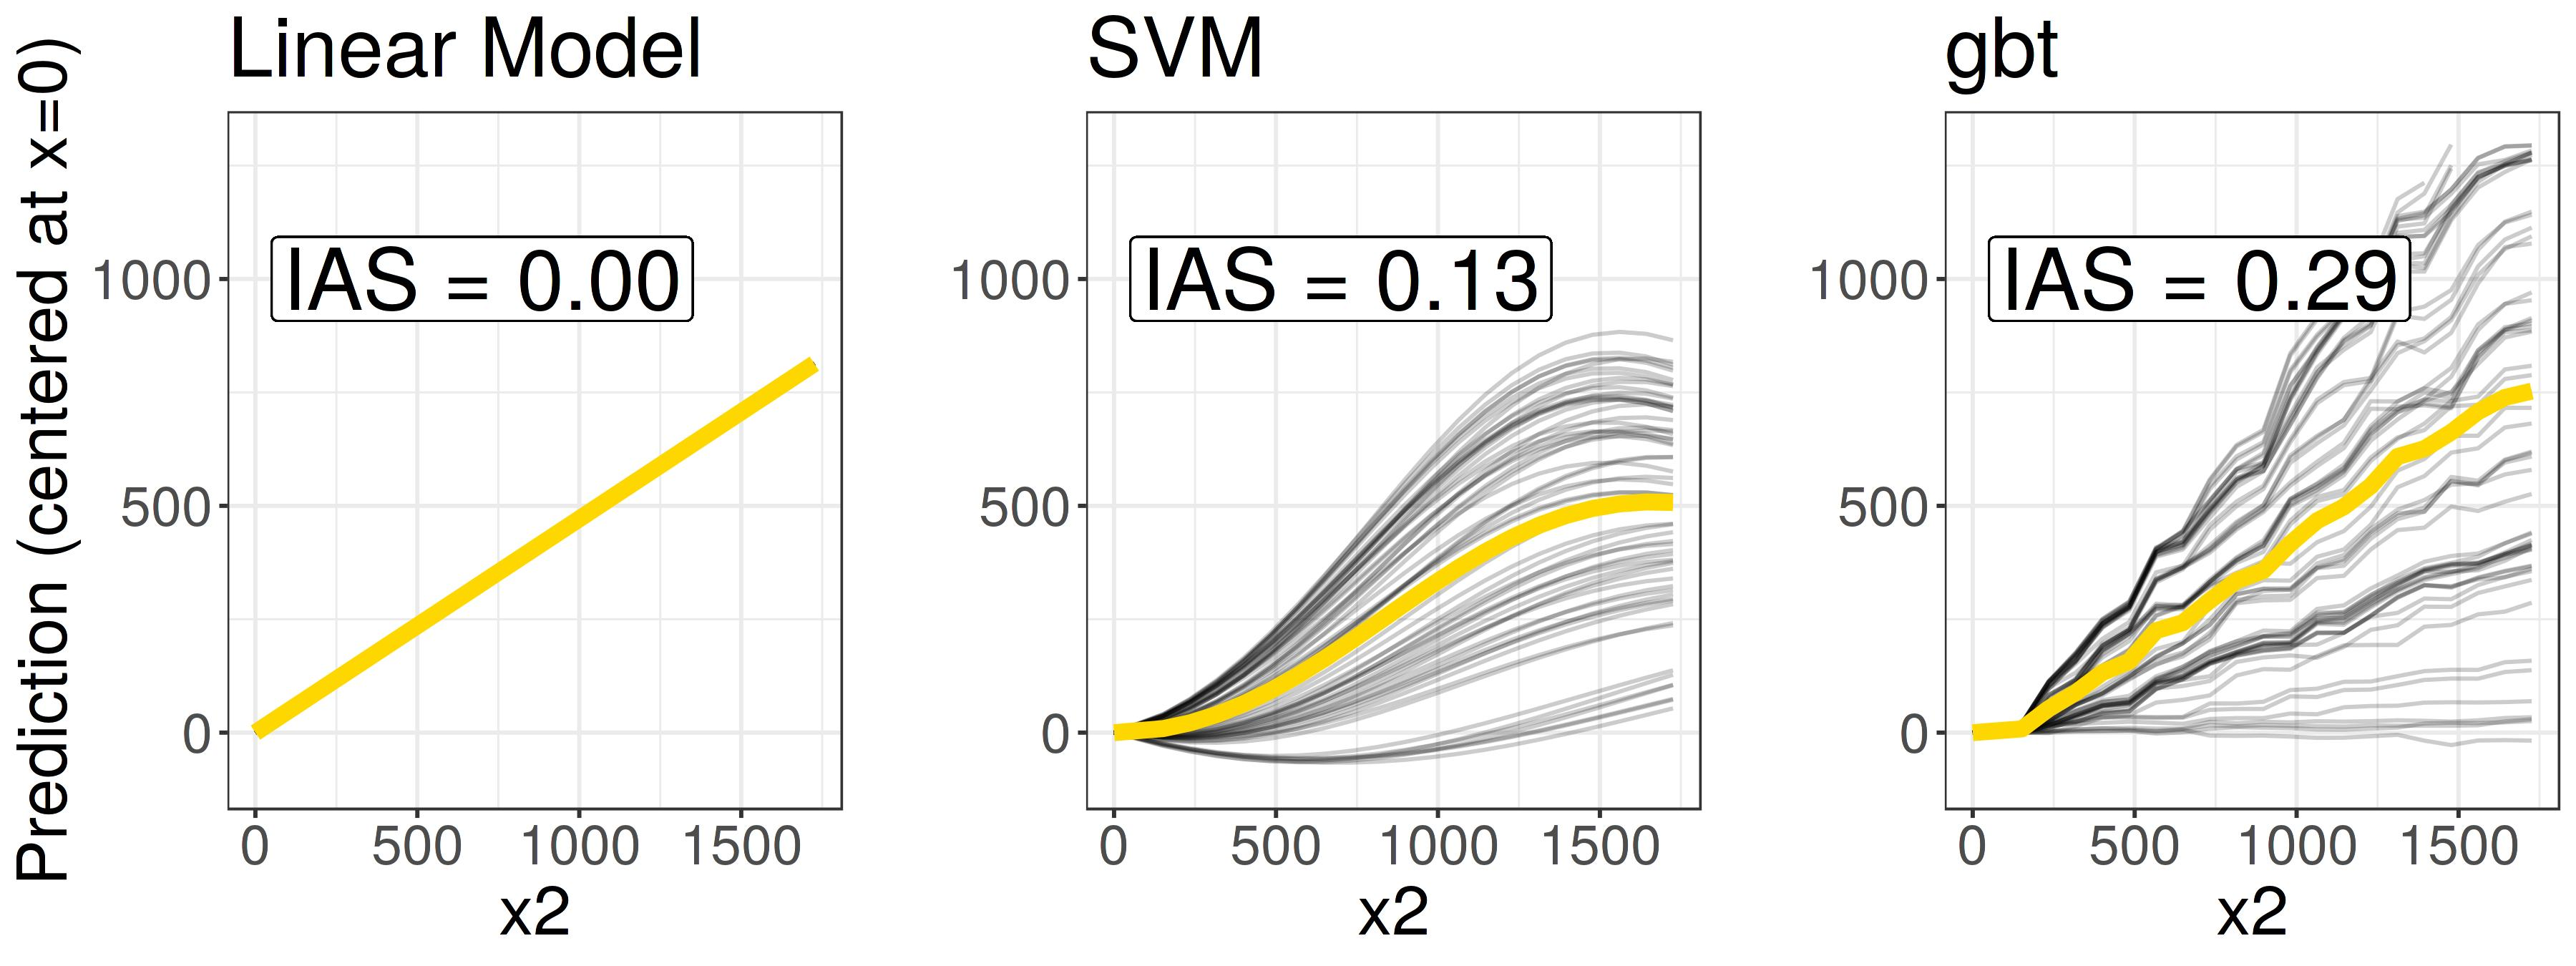
\includegraphics[width=12cm,height=4.5cm]{knit-fig/pdp-unreliable-1} 

}

\caption[The higher the interaction strength in a model (IAS increases from left to right), the less representative the Partial Dependence Plot (light thick line) becomes for individual instances represented by their Individual Conditional Expectation curves (dark thin lines)]{The higher the interaction strength in a model (IAS increases from left to right), the less representative the Partial Dependence Plot (light thick line) becomes for individual instances represented by their Individual Conditional Expectation curves (dark thin lines).}\label{fig:pdp-unreliable}
\end{figure}


\end{knitrout}



\textbf{The less complex the main effects, the better summarizable.}
In linear models, a feature effect can be expressed by a single number, the regression coefficient.
If effects are non-linear the method of choice is visualization  \citep{apley2016visualizing,friedman2001greedy}.
Summarizing the effects with a single number (e.g., using average marginal effects \citep{leeper2017interpreting}) can be misleading, e.g., the average effect might be zero for U-shaped feature effects.
As a by-product of MEC, there is a third option: Instead of reporting a single number, the coefficients of the segmented linear model can be reported.
Minimizing MEC means preferring models with main effects that can be described with fewer coefficients, offering a more compact model description.





\section{Application: Multi-objective Optimization}
\label{sec:multiobj}







%For all other parameters of the model-based, multi-objective optimization, we relied on the sensible defaults provided by \citep{mlrMBO}.
%
%\subsubsection{Model-based Optimization Setup.}
%We used the ParEGO algorithm \citep{knowles2006parego} for multi-objective optimization.
%Within the fitness function, the MAE was estimated using n.folds-fold cross-validation and the other measures (NF, MEC, IAS) were estimated using all data instances.
%We set the number of iterations of ParEGO to max.iters.
%

%
%
%

%

%
%

% =============================================================================
% Pareto Front Table
% =============================================================================
% =============================================================================
% Motivation for application
% =============================================================================
We demonstrate model selection for performance and complexity in a multi-objective optimization approach.
% =============================================================================
% Wine Data
% =============================================================================
%\subsubsection{Predicting Wine Quality.}
For this example, we predict wine quality (scale from 0 to 10) \citep{cortez2009modeling} from the wines physical-chemical properties such as alcohol and residual sugar of 4870 white wines.
% =============================================================================
% Why like this?
% =============================================================================
%\subsubsection{Motivation.}
It is difficult to know the desired compromise between model complexity and performance before modeling the data.
A solution is multi-objective optimization \citep{freitas2014comprehensible}.
We suggest searching over a wide spectrum of model classes and hyperparameter settings, which allows to select a suitable compromise between model complexity and performance.

% =============================================================================
% Objectives and Models
% =============================================================================
We used the mlrMBO model-based optimization framework \citep{horn2016multi} with ParEGO \citep{knowles2006parego} (500 iterations) to find the best models based on four objectives: number of features used (NF), main effect complexity (MEC), interaction strength (IAS) and cross-validated mean absolute error (MAE) (5-fold cross-validated).
We optimized over the space of following model classes (and hyperparameters): \textbf{CART} (maximum tree-depth and complexity parameter cp), \textbf{s}upport \textbf{v}ector \textbf{m}achine (cost C and inverse kernel width sigma), \textbf{elastic net} regression (regularization alpha and penalization lambda), \textbf{g}radient \textbf{b}oosted \textbf{t}rees (maximum depth, number of iterations), gradient \textbf{boost}ed \textbf{g}eneralized \textbf{a}dditive \textbf{m}odel (number of iterations nrounds) and \textbf{r}andom \textbf{f}orest (number of split features mtry).

\textbf{Results}.
The multi-objective optimization resulted in 27 models.
The measures had the following ranges: MAE 0.41 -- 0.63, number of features 1 --  11, mean effect complexity 1 -- 9 and interaction strength 0 -- 0.71.
For a more informative visualization, we propose to visualize the main effects together with the measures in Table~\ref{tab:spark-table-multiobj}.
The selected models show different trade-offs between the measures.
% =============================================================================
% Best performing model
% =============================================================================

% latex table generated in R 3.6.1 by xtable 1.8-4 package
% Mon Jul 29 13:10:38 2019
\begin{table}[ht]
\centering
\caption{A selection of four models from the Pareto optimal set, along with their ALE main effect curves. From left to right, the columns show models with 1) lowest MAE, 2) lowest MAE when $MEC=1$, 3) lowest MAE when $IAS =\leq 0.2$, and 4) lowest MAE with $NF \leq 7$.} 
\label{tab:spark-table-multiobj}
\begin{tabular}{l|p{2.2cm}p{2.2cm}p{2.2cm}p{2.2cm}}
  \hline
 & gbt (maxdepth:8, nrounds:269) & svm (C:23.6979, sigma:0.0003) & gbt (maxdepth:3, nrounds:98) & CART (maxdepth:14, cp:0.0074) \\ 
  \hline
MAE & 0.41 & 0.58 & 0.52 & 0.59 \\ 
  MEC & 4.2 & 1 & 4.5 & 2 \\ 
  IAS & 0.64 & 0 & 0.2 & 0.2 \\ 
  NF & 11 & 11 & 11 & 4 \\ 
  fixed.acidity & {\renewcommand{\sparklineheight}{3}\definecolor{sparklinecolor}{named}{black}\begin{sparkline}{10}
\spark 0 0.580723919439588 0.134615384615385 0.829992223699114 0.173076923076923 0.844456807214388 0.182692307692308 0.839682843980561 0.192307692307692 0.821612398859309 0.201923076923077 0.84542202787264 0.211538461538462 0.860259224728727 0.221153846153846 0.861102048282147 0.230769230769231 0.905582747874092 0.240384615384615 0.892915381185234 0.25 0.878589146536805 0.259615384615385 0.925284672477704 0.269230769230769 0.941678358605995 0.278846153846154 0.945197365201614 0.288461538461538 0.940126951520028 0.298076923076923 0.94825574011018 0.307692307692308 0.975399279836921 0.317307692307692 0.954553346609881 0.326923076923077 0.959445954007686 0.336538461538462 1 0.346153846153846 0.950705984625918 0.355769230769231 0.954262741269683 0.365384615384615 0.895767410489414 0.375 0.922568146288665 0.384615384615385 0.962892961969919 0.394230769230769 0.963828676235738 0.413461538461538 0.977723747818012 0.423076923076923 0.971038100486949 0.442307692307692 0.848911520533796 0.490384615384616 0.850986833558892 1 0 /
\end{sparkline}} & {\renewcommand{\sparklineheight}{3}\definecolor{sparklinecolor}{named}{black}\begin{sparkline}{10}
\spark 0 0 0.134615384615385 0.215570563451667 0.173076923076923 0.271311113886263 0.182692307692308 0.285888500154166 0.192307692307692 0.299690468134793 0.201923076923077 0.313664848832865 0.211538461538462 0.327516332414797 0.221153846153846 0.341452963105437 0.230769230769231 0.355437806420892 0.240384615384615 0.369358444207653 0.25 0.383243674200932 0.259615384615385 0.396698221641716 0.269230769230769 0.410175619486436 0.278846153846154 0.423332647993362 0.288461538461538 0.436602747059852 0.298076923076923 0.449442397527907 0.307692307692308 0.462156014508941 0.317307692307692 0.47462672157831 0.326923076923077 0.487277457866509 0.336538461538462 0.500145227151314 0.346153846153846 0.513015255595329 0.355769230769231 0.525236406014985 0.365384615384615 0.537308595705143 0.375 0.54913521610393 0.384615384615385 0.560676399193995 0.394230769230769 0.572118490583097 0.413461538461538 0.594565522962 0.423076923076923 0.604762710458392 0.442307692307692 0.625941784929779 0.490384615384616 0.674679686891622 1 1 /
\end{sparkline}} & {\renewcommand{\sparklineheight}{3}\definecolor{sparklinecolor}{named}{black}\begin{sparkline}{10}
\spark 0 0.844976539623567 0.134615384615385 0.889208299256031 0.173076923076923 0.860935019224948 0.182692307692308 0.822761364977456 0.192307692307692 0.822761364977456 0.201923076923077 0.822761364977456 0.211538461538462 0.822761364977456 0.221153846153846 0.822761364977456 0.230769230769231 0.888857479666717 0.240384615384615 0.887165307597015 0.25 0.887165307597015 0.259615384615385 0.908370713586534 0.269230769230769 0.896889062019068 0.278846153846154 0.90012699786746 0.288461538461538 0.90012699786746 0.298076923076923 0.898928350834181 0.307692307692308 0.979623308320354 0.317307692307692 0.935954758343701 0.326923076923077 0.935954758343701 0.336538461538462 1 0.346153846153846 0.915732047929759 0.355769230769231 0.816749422186957 0.365384615384615 0.780447872762861 0.375 0.842191668709934 0.384615384615385 0.842191668709934 0.394230769230769 0.842191668709934 0.413461538461538 0.882199614001737 0.423076923076923 0.813642509233885 0.442307692307692 0.667966284620276 0.490384615384616 0.667966284620276 1 0 /
\end{sparkline}} &  \\ 
  volatile.acidity & {\renewcommand{\sparklineheight}{3}\definecolor{sparklinecolor}{named}{black}\begin{sparkline}{10}
\spark 0 0.976117779372163 0.0490196078431373 1 0.0686274509803921 0.932439787788862 0.0784313725490196 0.9057205186278 0.0882352941176471 0.89904295070012 0.0980392156862745 0.928769291975546 0.107843137254902 0.935759101011661 0.117647058823529 0.831645481942826 0.127450980392157 0.799444128463582 0.137254901960784 0.787148998276219 0.147058823529412 0.792859015976838 0.156862745098039 0.730008563450883 0.166666666666667 0.742458471460207 0.176470588235294 0.666466169207774 0.186274509803922 0.663152747642992 0.196078431372549 0.641578763516196 0.205882352941176 0.645501550691957 0.215686274509804 0.686123472206636 0.225490196078431 0.599044157431634 0.235294117647059 0.582625926064704 0.245098039215686 0.585062459453443 0.254901960784314 0.620364993613008 0.264705882352941 0.641958174886897 0.274509803921569 0.638540980713387 0.284313725490196 0.621944094864603 0.294117647058824 0.601873916980047 0.313725490196078 0.626512069924011 0.333333333333333 0.658052945995492 0.352941176470588 0.713165186179756 0.392156862745098 0.643013191039153 0.470588235294118 0.50641886295964 1 0 /
\end{sparkline}} & {\renewcommand{\sparklineheight}{3}\definecolor{sparklinecolor}{named}{black}\begin{sparkline}{10}
\spark 0 1 0.0490196078431373 0.948986967370644 0.0686274509803921 0.928557220897754 0.0784313725490196 0.918304525607617 0.0882352941176471 0.908106495878793 0.0980392156862745 0.897810088771018 0.107843137254902 0.88751180277117 0.117647058823529 0.877290904765281 0.127450980392157 0.867061615960346 0.137254901960784 0.856770374716112 0.147058823529412 0.84641923857144 0.156862745098039 0.836185117917192 0.166666666666667 0.825856682013202 0.176470588235294 0.815587699044824 0.186274509803922 0.805339856852975 0.196078431372549 0.79509393520449 0.205882352941176 0.784872921998428 0.215686274509804 0.774702591482917 0.225490196078431 0.764509182892903 0.235294117647059 0.754376397381746 0.245098039215686 0.744243544860019 0.254901960784314 0.73406073859078 0.264705882352941 0.723870026980678 0.274509803921569 0.713813329825559 0.284313725490196 0.703759946517018 0.294117647058824 0.69362551258752 0.313725490196078 0.673393891094531 0.333333333333333 0.653271142602105 0.352941176470588 0.633162449660739 0.392156862745098 0.593347851747841 0.470588235294118 0.513499415953113 1 0 /
\end{sparkline}} & {\renewcommand{\sparklineheight}{3}\definecolor{sparklinecolor}{named}{black}\begin{sparkline}{10}
\spark 0 1 0.0490196078431373 0.928850661412978 0.0686274509803921 0.873518517566659 0.0784313725490196 0.824793081188484 0.0882352941176471 0.824793081188484 0.0980392156862745 0.824793081188484 0.107843137254902 0.80694891229943 0.117647058823529 0.762258787301009 0.127450980392157 0.623682068139692 0.137254901960784 0.643637883087249 0.147058823529412 0.643637883087249 0.156862745098039 0.610028434064757 0.166666666666667 0.611050593941929 0.176470588235294 0.542413760348095 0.186274509803922 0.541635675415188 0.196078431372549 0.541937794724689 0.205882352941176 0.503500555422228 0.215686274509804 0.501572982795931 0.225490196078431 0.465143097914243 0.235294117647059 0.465143097914243 0.245098039215686 0.481219473354096 0.254901960784314 0.478743776100525 0.264705882352941 0.478743776100525 0.274509803921569 0.478743776100525 0.284313725490196 0.478743776100525 0.294117647058824 0.451878335565322 0.313725490196078 0.451878335565322 0.333333333333333 0.499659513594882 0.352941176470588 0.559757404375537 0.392156862745098 0.412989331297578 0.470588235294118 0.258012687136739 1 0 /
\end{sparkline}} & {\renewcommand{\sparklineheight}{3}\definecolor{sparklinecolor}{named}{black}\begin{sparkline}{10}
\spark 0 1 0.0490196078431373 1 0.0686274509803921 1 0.0784313725490196 1 0.0882352941176471 1 0.0980392156862745 1 0.107843137254902 1 0.117647058823529 1 0.127450980392157 0.629240796739237 0.137254901960784 0.629240796739237 0.147058823529412 0.629240796739237 0.156862745098039 0.629240796739237 0.166666666666667 0.629240796739237 0.176470588235294 0.244325967797506 0.186274509803922 0.244325967797506 0.196078431372549 0.244325967797506 0.205882352941176 0.244325967797506 0.215686274509804 0.244325967797506 0.225490196078431 0.244325967797506 0.235294117647059 0.244325967797506 0.245098039215686 0.244325967797506 0.254901960784314 0.244325967797506 0.264705882352941 0.244325967797506 0.274509803921569 0.244325967797506 0.284313725490196 0.244325967797506 0.294117647058824 0.244325967797506 0.313725490196078 0.244325967797506 0.333333333333333 0.244325967797506 0.352941176470588 0.244325967797506 0.392156862745098 0 0.470588235294118 0 1 0 /
\end{sparkline}} \\ 
  citric.acid & {\renewcommand{\sparklineheight}{3}\definecolor{sparklinecolor}{named}{black}\begin{sparkline}{10}
\spark 0 0 0.0662650602409639 0.278554631390282 0.0963855421686747 0.491085859863838 0.114457831325301 0.326634187458365 0.120481927710843 0.400681385162273 0.132530120481928 0.453482402639508 0.13855421686747 0.471694062911795 0.144578313253012 0.623341438558108 0.150602409638554 0.67091057210913 0.156626506024096 0.698792015143804 0.162650602409639 0.917732519376424 0.168674698795181 0.930744434690728 0.174698795180723 0.919609343648825 0.180722891566265 0.928734494109734 0.186746987951807 1 0.192771084337349 0.978016063019647 0.198795180722892 0.963863733926575 0.204819277108434 0.878488307349148 0.210843373493976 0.881258018958058 0.216867469879518 0.939522215327548 0.22289156626506 0.803321316650486 0.228915662650602 0.857435161629435 0.234939759036145 0.94666853973578 0.240963855421687 0.903418852575778 0.246987951807229 0.798236376851575 0.253012048192771 0.877271806111093 0.265060240963855 0.821207110001061 0.27710843373494 0.79797995853352 0.289156626506024 0.89968309802311 0.295180722891566 0.897404146601734 0.307228915662651 0.803853118523366 0.343373493975904 0.81075151040921 0.403614457831325 0.773387059964341 1 0.488074453763928 /
\end{sparkline}} & {\renewcommand{\sparklineheight}{3}\definecolor{sparklinecolor}{named}{black}\begin{sparkline}{10}
\spark 0 0.972052713530984 0.0662650602409639 0.993661163539371 0.0963855421686747 0.998478003651821 0.114457831325301 0.99979806439297 0.120481927710843 0.999993032032751 0.132530120481928 1 0.13855421686747 0.99979539407633 0.144578313253012 0.999569182291352 0.150602409638554 0.999179838912073 0.156626506024096 0.998610260982236 0.162650602409639 0.998030623333776 0.168674698795181 0.997199749328538 0.174698795180723 0.996350771788666 0.180722891566265 0.995413455795488 0.186746987951807 0.99429270482724 0.192771084337349 0.993157018015645 0.198795180722892 0.991901398464648 0.204819277108434 0.990452006261148 0.210843373493976 0.988886193114679 0.216867469879518 0.987115413358173 0.22289156626506 0.985328949113297 0.228915662650602 0.983593884900552 0.234939759036145 0.981732538506895 0.240963855421687 0.979650340368633 0.246987951807229 0.977271970013224 0.253012048192771 0.974908910668043 0.265060240963855 0.969975619278456 0.27710843373494 0.964796961142969 0.289156626506024 0.959377972346215 0.295180722891566 0.956364622016304 0.307228915662651 0.950080722591885 0.343373493975904 0.929513462509021 0.403614457831325 0.886334295298319 1 0 /
\end{sparkline}} & {\renewcommand{\sparklineheight}{3}\definecolor{sparklinecolor}{named}{black}\begin{sparkline}{10}
\spark 0 0 0.0662650602409639 0.31923577815926 0.0963855421686747 0.63649336775669 0.114457831325301 0.512546781896585 0.120481927710843 0.512546781896585 0.132530120481928 0.512546781896585 0.13855421686747 0.512546781896585 0.144578313253012 0.743998389050424 0.150602409638554 0.738501756691808 0.156626506024096 0.762786133879742 0.162650602409639 1 0.168674698795181 0.99689755657763 0.174698795180723 0.981884563682681 0.180722891566265 0.927080246470186 0.186746987951807 0.927080246470186 0.192771084337349 0.927080246470186 0.198795180722892 0.939002129956611 0.204819277108434 0.939002129956611 0.210843373493976 0.885368734256462 0.216867469879518 0.93401061149688 0.22289156626506 0.786985770796039 0.228915662650602 0.794094658218737 0.234939759036145 0.794094658218737 0.240963855421687 0.794094658218737 0.246987951807229 0.795384212625018 0.253012048192771 0.795384212625018 0.265060240963855 0.795384212625018 0.27710843373494 0.490557277677136 0.289156626506024 0.653598772998526 0.295180722891566 0.839584264762518 0.307228915662651 0.839584264762518 0.343373493975904 0.73611085647023 0.403614457831325 0.73611085647023 1 0.394789569236506 /
\end{sparkline}} &  \\ 
  residual.sugar & {\renewcommand{\sparklineheight}{3}\definecolor{sparklinecolor}{named}{black}\begin{sparkline}{10}
\spark 0 0 0.00613496932515337 0.505537351514397 0.00766871165644172 0.52399503389013 0.00920245398773006 0.498075409852005 0.0107361963190184 0.542928213804944 0.0122699386503067 0.570430044247915 0.0138036809815951 0.583035906057885 0.0153374233128834 0.582296572471391 0.0168711656441718 0.563829265416184 0.0184049079754601 0.565008523764531 0.0199386503067485 0.575731844393911 0.0214723926380368 0.581538022501428 0.0245398773006135 0.669326479968024 0.0276073619631902 0.673487771271201 0.0322085889570552 0.662892362571054 0.0352760736196319 0.61994396904537 0.0429447852760736 0.646276846640952 0.0506134969325153 0.640410838547 0.0567484662576687 0.67752258242118 0.0613496932515337 0.706473394132816 0.0659509202453988 0.693296034201664 0.0705521472392638 0.678341102938146 0.0782208588957055 0.673110934982158 0.0828220858895706 0.67697600816213 0.0889570552147239 0.66459816783164 0.093558282208589 0.690047162094248 0.098159509202454 0.761206536136408 0.104294478527607 0.785834420690848 0.108895705521472 0.759598028180513 0.111963190184049 0.74186236448857 0.116564417177914 0.727622768428662 0.122699386503067 0.718062509292668 0.128834355828221 0.776158505820692 0.138803680981595 0.775511083821051 0.147239263803681 0.843808296464972 0.153374233128834 0.843085899517059 0.162576687116564 0.837117452340984 0.171779141104294 0.777816462828445 0.179447852760736 0.896924203170337 0.187116564417178 0.931282682156365 0.19478527607362 0.929884002469266 0.205521472392638 1 0.213957055214724 0.904717243737015 0.226993865030675 0.779239157034119 0.242331288343558 0.77763556501212 0.263803680981595 0.848303187210467 1 0.720743355387846 /
\end{sparkline}} & {\renewcommand{\sparklineheight}{3}\definecolor{sparklinecolor}{named}{black}\begin{sparkline}{10}
\spark 0 0 0.00613496932515337 0.00655105833915008 0.00766871165644172 0.00818478440210957 0.00920245398773006 0.00981714804281547 0.0107361963190184 0.0114447324226774 0.0122699386503067 0.0130728281248936 0.0138036809815951 0.0147020482920296 0.0153374233128834 0.0163318181584077 0.0168711656441718 0.0179543536990215 0.0184049079754601 0.0195801995189908 0.0199386503067485 0.0212065110860464 0.0214723926380368 0.0228346754413199 0.0245398773006135 0.0260845560167569 0.0276073619631902 0.0293385119630664 0.0322085889570552 0.0342087458484097 0.0352760736196319 0.0374530301664653 0.0429447852760736 0.0455969039581771 0.0506134969325153 0.0537259946314746 0.0567484662576687 0.0602194114159275 0.0613496932515337 0.0650804574803097 0.0659509202453988 0.0699443159287502 0.0705521472392638 0.0748147497629572 0.0782208588957055 0.0829342037187663 0.0828220858895706 0.0878035868023446 0.0889570552147239 0.0942871579071698 0.093558282208589 0.0991470460110789 0.098159509202454 0.103996700685986 0.104294478527607 0.110478993126781 0.108895705521472 0.115314512080301 0.111963190184049 0.118547646802455 0.116564417177914 0.123393777408704 0.122699386503067 0.129855363679618 0.128834355828221 0.136336296075782 0.138803680981595 0.146886184198267 0.147239263803681 0.155787555606533 0.153374233128834 0.162257451966915 0.162576687116564 0.171957906168694 0.171779141104294 0.1816301001721 0.179447852760736 0.18966211620922 0.187116564417178 0.197718195209057 0.19478527607362 0.205741725224615 0.205521472392638 0.217041526669193 0.213957055214724 0.225921511028302 0.226993865030675 0.239648429449301 0.242331288343558 0.255734401195063 0.263803680981595 0.278282998972399 1 1 /
\end{sparkline}} & {\renewcommand{\sparklineheight}{3}\definecolor{sparklinecolor}{named}{black}\begin{sparkline}{10}
\spark 0 0 0.00613496932515337 0.403441122271154 0.00766871165644172 0.407218463526097 0.00920245398773006 0.398251567316897 0.0107361963190184 0.441390469210787 0.0122699386503067 0.484940321379439 0.0138036809815951 0.484940321379439 0.0153374233128834 0.484940321379439 0.0168711656441718 0.48189781306549 0.0184049079754601 0.507260266370697 0.0199386503067485 0.507260266370697 0.0214723926380368 0.507260266370697 0.0245398773006135 0.584472018159758 0.0276073619631902 0.597460182923216 0.0322085889570552 0.58179771461023 0.0352760736196319 0.58179771461023 0.0429447852760736 0.58179771461023 0.0506134969325153 0.602339029833986 0.0567484662576687 0.602339029833986 0.0613496932515337 0.602339029833986 0.0659509202453988 0.602339029833986 0.0705521472392638 0.599680566204361 0.0782208588957055 0.617178426445403 0.0828220858895706 0.617178426445403 0.0889570552147239 0.617178426445403 0.093558282208589 0.619779481778635 0.098159509202454 0.633702550661302 0.104294478527607 0.64629552593595 0.108895705521472 0.64629552593595 0.111963190184049 0.649004176478869 0.116564417177914 0.649004176478869 0.122699386503067 0.654716253962481 0.128834355828221 0.675699988965846 0.138803680981595 0.669717907351133 0.147239263803681 0.698117384435471 0.153374233128834 0.698117384435471 0.162576687116564 0.690785007534411 0.171779141104294 0.690785007534411 0.179447852760736 0.696395987995268 0.187116564417178 0.798449779775842 0.19478527607362 0.798449779775842 0.205521472392638 1 0.213957055214724 0.81645273242206 0.226993865030675 0.675390642171884 0.242331288343558 0.607465899257019 0.263803680981595 0.716640933608999 1 0.601551414193347 /
\end{sparkline}} &  \\ 
  chlorides & {\renewcommand{\sparklineheight}{3}\definecolor{sparklinecolor}{named}{black}\begin{sparkline}{10}
\spark 0 0 0.0415430267062315 0.919764458118848 0.0504451038575668 0.913914855597416 0.056379821958457 0.939918914365498 0.0593471810089021 0.952799702391384 0.0623145400593472 0.947516796364497 0.0652818991097923 0.984994278909757 0.0682492581602374 0.940276192740545 0.0712166172106825 0.911073505864237 0.0741839762611276 0.922330858288531 0.0771513353115727 0.930470565622124 0.0801186943620178 0.977679393436983 0.0830860534124629 1 0.086053412462908 0.947647104132623 0.0890207715133531 0.989672507865471 0.0919881305637982 0.844808348448411 0.0949554896142433 0.845412392022845 0.0979228486646884 0.837705083348357 0.100890207715134 0.834429986690094 0.103857566765579 0.869532605707813 0.106824925816024 0.786837934166755 0.109792284866469 0.781853982764112 0.112759643916914 0.797593352475147 0.115727002967359 0.823984536312125 0.118694362017804 0.837020033321961 0.121661721068249 0.708795171088165 0.124629080118694 0.624054441512955 0.127596439169139 0.636929736360521 0.130563798219585 0.671821410939979 0.13353115727003 0.660825722051075 0.136498516320475 0.688589860149494 0.13946587537092 0.724205412562782 0.14540059347181 0.756819705757591 0.1513353115727 0.661981362347119 0.163204747774481 0.535035455018343 0.189910979228487 0.539754758977188 0.320474777448071 0.818810186081235 1 0.662257854394562 /
\end{sparkline}} & {\renewcommand{\sparklineheight}{3}\definecolor{sparklinecolor}{named}{black}\begin{sparkline}{10}
\spark 0 1 0.0415430267062315 0.88101569172914 0.0504451038575668 0.855886025457219 0.056379821958457 0.839320945006189 0.0593471810089021 0.83103559283293 0.0623145400593472 0.822643277707214 0.0652818991097923 0.814446723985582 0.0682492581602374 0.806327807613496 0.0712166172106825 0.798223418052451 0.0741839762611276 0.790130719395729 0.0771513353115727 0.782184023528779 0.0801186943620178 0.77407292392524 0.0830860534124629 0.766311780734109 0.086053412462908 0.758405220849333 0.0890207715133531 0.750586443255762 0.0919881305637982 0.742787453852346 0.0949554896142433 0.735088650175668 0.0979228486646884 0.727549603754603 0.100890207715134 0.719914413253786 0.103857566765579 0.712305750623491 0.106824925816024 0.704972228761895 0.109792284866469 0.697393509826705 0.112759643916914 0.689913780744743 0.115727002967359 0.682363825593847 0.118694362017804 0.674982644490769 0.121661721068249 0.667915501939129 0.124629080118694 0.660416763273343 0.127596439169139 0.653182013491935 0.130563798219585 0.645815020366723 0.13353115727003 0.638553149038656 0.136498516320475 0.631288904933125 0.13946587537092 0.624452854869772 0.14540059347181 0.610475859200586 0.1513353115727 0.59589797219658 0.163204747774481 0.568234302557486 0.189910979228487 0.507097159827643 0.320474777448071 0.244837188917112 1 0 /
\end{sparkline}} & {\renewcommand{\sparklineheight}{3}\definecolor{sparklinecolor}{named}{black}\begin{sparkline}{10}
\spark 0 0.675156787477266 0.0415430267062315 0.962335608760995 0.0504451038575668 0.789372317372563 0.056379821958457 0.982149871803726 0.0593471810089021 0.962656158445986 0.0623145400593472 0.914494895579489 0.0652818991097923 0.914494895579489 0.0682492581602374 0.914494895579489 0.0712166172106825 0.968451571996495 0.0741839762611276 1 0.0771513353115727 1 0.0801186943620178 1 0.0830860534124629 1 0.086053412462908 0.950346508772842 0.0890207715133531 0.920704082854389 0.0919881305637982 0.584454782606496 0.0949554896142433 0.606019889636725 0.0979228486646884 0.606019889636725 0.100890207715134 0.606019889636725 0.103857566765579 0.62099559730429 0.106824925816024 0.542237030335734 0.109792284866469 0.562550977080885 0.112759643916914 0.562550977080885 0.115727002967359 0.562550977080885 0.118694362017804 0.562550977080885 0.121661721068249 0.310946324593899 0.124629080118694 0.229596519875743 0.127596439169139 0.229596519875743 0.130563798219585 0.210777989135365 0.13353115727003 0.210777989135365 0.136498516320475 0.322352872011517 0.13946587537092 0.322352872011517 0.14540059347181 0.322352872011517 0.1513353115727 0.322352872011517 0.163204747774481 0.238640500502638 0.189910979228487 0.238640500502638 0.320474777448071 0.851765813546818 1 0 /
\end{sparkline}} &  \\ 
  free.sulfur.dioxide & {\renewcommand{\sparklineheight}{3}\definecolor{sparklinecolor}{named}{black}\begin{sparkline}{10}
\spark 0 0 0.0174216027874564 0.319862907253727 0.0278745644599303 0.356262473826538 0.0348432055749129 0.621306247738202 0.0418118466898955 0.671952799051417 0.0452961672473868 0.664566901605259 0.0522648083623693 0.660889267051274 0.0557491289198606 0.664242655659092 0.0592334494773519 0.698508872051188 0.0627177700348432 0.705535783889333 0.0662020905923345 0.70639529543578 0.0696864111498258 0.7675056617706 0.0731707317073171 0.755834370634729 0.0766550522648084 0.742136761933418 0.0801393728222996 0.819832796295295 0.0836236933797909 0.846837476510877 0.0871080139372822 0.832972168629698 0.0905923344947735 0.859475628522591 0.0940766550522648 0.886149721540358 0.0975609756097561 0.930916276296169 0.101045296167247 0.917673545837486 0.104529616724739 0.914220248386065 0.10801393728223 0.924105452659259 0.111498257839721 0.865300241556187 0.114982578397213 0.898890531219341 0.118466898954704 0.918164538649237 0.121951219512195 0.920753542909247 0.125435540069686 0.905803398168923 0.128919860627178 0.945539393312262 0.132404181184669 0.934093767700653 0.13588850174216 0.958008106243322 0.139372822299652 0.940839707227538 0.142857142857143 0.957613119889063 0.146341463414634 0.972068486854265 0.149825783972125 0.975148608426991 0.156794425087108 0.970861652421419 0.160278745644599 0.963812290695821 0.163763066202091 0.975792957627334 0.167247386759582 0.976497826006349 0.174216027874564 0.981632966428979 0.177700348432056 1 0.184668989547038 0.948219894279362 0.191637630662021 0.936124378056002 0.198606271777003 0.953672029677399 0.209059233449477 0.997449757727631 0.222996515679443 0.993712673952852 0.24390243902439 0.971211679007026 1 0.332747676394517 /
\end{sparkline}} & {\renewcommand{\sparklineheight}{3}\definecolor{sparklinecolor}{named}{black}\begin{sparkline}{10}
\spark 0 0 0.0174216027874564 0.08337673854884 0.0278745644599303 0.130677659026026 0.0348432055749129 0.162308892935692 0.0418118466898955 0.193517121290914 0.0452961672473868 0.209017905643178 0.0522648083623693 0.239410955066682 0.0557491289198606 0.254546787922358 0.0592334494773519 0.269489052531077 0.0627177700348432 0.284419829018214 0.0662020905923345 0.299024701176908 0.0696864111498258 0.313501045958959 0.0731707317073171 0.328036183975251 0.0766550522648084 0.342434328774849 0.0801393728222996 0.356585751693592 0.0836236933797909 0.370746509507367 0.0871080139372822 0.384773231791864 0.0905923344947735 0.398596893558152 0.0940766550522648 0.412397238481744 0.0975609756097561 0.42631522828023 0.101045296167247 0.440072769875176 0.104529616724739 0.453438689079102 0.10801393728223 0.466638474118815 0.111498257839721 0.479955223827283 0.114982578397213 0.492821381364137 0.118466898954704 0.505871033488555 0.121951219512195 0.518723928742695 0.125435540069686 0.531682318698624 0.128919860627178 0.544444490547262 0.132404181184669 0.557101440739227 0.13588850174216 0.569461567367717 0.139372822299652 0.581604478010767 0.142857142857143 0.593849478622089 0.146341463414634 0.605521542136272 0.149825783972125 0.61719659631369 0.156794425087108 0.640466516800082 0.160278745644599 0.65168053026258 0.163763066202091 0.662842212916803 0.167247386759582 0.673835971592235 0.174216027874564 0.695561215293257 0.177700348432056 0.706057828507809 0.184668989547038 0.726696756422238 0.191637630662021 0.747407242097904 0.198606271777003 0.767527730250028 0.209059233449477 0.797152152266349 0.222996515679443 0.83566623952673 0.24390243902439 0.890206276830521 1 1 /
\end{sparkline}} & {\renewcommand{\sparklineheight}{3}\definecolor{sparklinecolor}{named}{black}\begin{sparkline}{10}
\spark 0 0.18495216651729 0.0174216027874564 0.429153976524003 0.0278745644599303 0.490787941439488 0.0348432055749129 0.716365273457623 0.0418118466898955 0.801139647568664 0.0452961672473868 0.792193120838717 0.0522648083623693 0.788491531708487 0.0557491289198606 0.801113717792305 0.0592334494773519 0.808466149874415 0.0627177700348432 0.803485739595662 0.0662020905923345 0.84986387342483 0.0696864111498258 0.86279817170191 0.0731707317073171 0.86279817170191 0.0766550522648084 0.867129501420484 0.0801393728222996 0.94596741637343 0.0836236933797909 0.94596741637343 0.0871080139372822 0.94596741637343 0.0905923344947735 0.962309556885424 0.0940766550522648 0.988256776021792 0.0975609756097561 0.985522235675332 0.101045296167247 0.985522235675332 0.104529616724739 0.991457115874824 0.10801393728223 0.991457115874824 0.111498257839721 0.991457115874824 0.114982578397213 0.991457115874824 0.118466898954704 0.991457115874824 0.121951219512195 0.991457115874824 0.125435540069686 0.986927551800695 0.128919860627178 0.998560301021468 0.132404181184669 0.998560301021468 0.13588850174216 0.998560301021468 0.139372822299652 0.998560301021468 0.142857142857143 0.998560301021468 0.146341463414634 0.983354959923589 0.149825783972125 0.989396072911386 0.156794425087108 0.989396072911386 0.160278745644599 0.989396072911386 0.163763066202091 0.989396072911386 0.167247386759582 0.989396072911386 0.174216027874564 0.996681617677463 0.177700348432056 0.996681617677463 0.184668989547038 0.993606324762868 0.191637630662021 1 0.198606271777003 0.986649985358008 0.209059233449477 0.972100969304973 0.222996515679443 0.972100969304973 0.24390243902439 0.972100969304973 1 0 /
\end{sparkline}} & {\renewcommand{\sparklineheight}{3}\definecolor{sparklinecolor}{named}{black}\begin{sparkline}{10}
\spark 0 0 0.0174216027874564 0 0.0278745644599303 0 0.0348432055749129 0.771620810573821 0.0418118466898955 0.771620810573821 0.0452961672473868 0.771620810573821 0.0522648083623693 0.771620810573821 0.0557491289198606 1 0.0592334494773519 1 0.0627177700348432 1 0.0662020905923345 1 0.0696864111498258 1 0.0731707317073171 1 0.0766550522648084 1 0.0801393728222996 1 0.0836236933797909 1 0.0871080139372822 1 0.0905923344947735 1 0.0940766550522648 1 0.0975609756097561 1 0.101045296167247 1 0.104529616724739 1 0.10801393728223 1 0.111498257839721 1 0.114982578397213 1 0.118466898954704 1 0.121951219512195 1 0.125435540069686 1 0.128919860627178 1 0.132404181184669 1 0.13588850174216 1 0.139372822299652 1 0.142857142857143 1 0.146341463414634 1 0.149825783972125 1 0.156794425087108 1 0.160278745644599 1 0.163763066202091 1 0.167247386759582 1 0.174216027874564 1 0.177700348432056 1 0.184668989547038 1 0.191637630662021 1 0.198606271777003 1 0.209059233449477 1 0.222996515679443 1 0.24390243902439 1 1 1 /
\end{sparkline}} \\ 
  total.sulfur.dioxide & {\renewcommand{\sparklineheight}{3}\definecolor{sparklinecolor}{named}{black}\begin{sparkline}{10}
\spark 0 0 0.122969837587007 0.552100793378045 0.146171693735499 0.711333477001614 0.160092807424594 0.73327299422107 0.17169373549884 0.809005024945026 0.180974477958237 0.723266180459614 0.190255220417633 0.773171663852432 0.197215777262181 0.918535428808879 0.204176334106729 1 0.208816705336427 0.88871752309914 0.215777262180974 0.716681381666076 0.220417633410673 0.754928315222125 0.22737819025522 0.800568695661374 0.234338747099768 0.812701159808464 0.236658932714617 0.812811020909294 0.241299303944316 0.887547253368665 0.245939675174014 0.862927444617398 0.250580046403712 0.848771413365434 0.255220417633411 0.8537154234068 0.259860788863109 0.824389262257771 0.266821345707657 0.874509582585451 0.271461716937355 0.849774919849528 0.276102088167053 0.878528064384847 0.280742459396752 0.88899589495165 0.28538283062645 0.749037446377675 0.290023201856148 0.760872569677911 0.294663573085847 0.710190334340565 0.301624129930394 0.711425851794603 0.308584686774942 0.723613635461207 0.31322505800464 0.644867347963935 0.320185614849188 0.65838794666342 0.324825986078886 0.667982058477783 0.331786542923434 0.721953193719454 0.338747099767981 0.724505120016984 0.34338747099768 0.699344448404779 0.350348027842227 0.666736316391314 0.357308584686775 0.63507658522271 0.364269141531323 0.681425030614525 0.368909512761021 0.670509892458436 0.378190255220418 0.603255308597443 0.387470997679814 0.522441311250905 0.394431554524362 0.625086719905799 0.40139211136891 0.553189307707689 0.410672853828306 0.582339472927063 0.419953596287703 0.612445642145042 0.431554524361949 0.579080857426323 0.443155452436195 0.489600784362061 0.464037122969838 0.690730258556146 0.480278422273782 0.593972875616711 0.510440835266821 0.651421018840022 1 0.433875627462003 /
\end{sparkline}} & {\renewcommand{\sparklineheight}{3}\definecolor{sparklinecolor}{named}{black}\begin{sparkline}{10}
\spark 0 1 0.122969837587007 0.959445863444689 0.146171693735499 0.948948995370033 0.160092807424594 0.942120984559463 0.17169373549884 0.936190524590442 0.180974477958237 0.931360586487506 0.190255220417633 0.926149448588144 0.197215777262181 0.922212130655022 0.204176334106729 0.918195261571634 0.208816705336427 0.915514858576103 0.215777262180974 0.911405672728568 0.220417633410673 0.908514710563569 0.22737819025522 0.904172186563202 0.234338747099768 0.899791971890926 0.236658932714617 0.898311435350491 0.241299303944316 0.895285790702128 0.245939675174014 0.892213226928453 0.250580046403712 0.889151056407726 0.255220417633411 0.886083289780897 0.259860788863109 0.882926004826771 0.266821345707657 0.878225602861442 0.271461716937355 0.875109904040166 0.276102088167053 0.871780987354663 0.280742459396752 0.868423517144726 0.28538283062645 0.865169389428573 0.290023201856148 0.861685828765741 0.294663573085847 0.858308255503351 0.301624129930394 0.85310350225323 0.308584686774942 0.847757746649748 0.31322505800464 0.844189090636048 0.320185614849188 0.838614152825915 0.324825986078886 0.83493118340593 0.331786542923434 0.829240772463841 0.338747099767981 0.823427304285061 0.34338747099768 0.819654807973638 0.350348027842227 0.813709794179918 0.357308584686775 0.807693113076391 0.364269141531323 0.801768394322382 0.368909512761021 0.79774778746056 0.378190255220418 0.789457192283386 0.387470997679814 0.781090024355785 0.394431554524362 0.774646463597224 0.40139211136891 0.768265225637878 0.410672853828306 0.759422671368361 0.419953596287703 0.750593543500225 0.431554524361949 0.73956142142063 0.443155452436195 0.728027470909417 0.464037122969838 0.706792650331223 0.480278422273782 0.689836247411278 0.510440835266821 0.657867888025837 1 0 /
\end{sparkline}} & {\renewcommand{\sparklineheight}{3}\definecolor{sparklinecolor}{named}{black}\begin{sparkline}{10}
\spark 0 1 0.122969837587007 0.507665610722905 0.146171693735499 0.656459430984023 0.160092807424594 0.631166323700183 0.17169373549884 0.647049138570866 0.180974477958237 0.647049138570866 0.190255220417633 0.678348342339531 0.197215777262181 0.706610822340971 0.204176334106729 0.706610822340971 0.208816705336427 0.67131264629326 0.215777262180974 0.624720649483767 0.220417633410673 0.624720649483767 0.22737819025522 0.640587526444699 0.234338747099768 0.640587526444699 0.236658932714617 0.640587526444699 0.241299303944316 0.677564499150452 0.245939675174014 0.674928435866846 0.250580046403712 0.674928435866846 0.255220417633411 0.674928435866846 0.259860788863109 0.674928435866846 0.266821345707657 0.674928435866846 0.271461716937355 0.674928435866846 0.276102088167053 0.672394063899651 0.280742459396752 0.672394063899651 0.28538283062645 0.644414988573057 0.290023201856148 0.644414988573057 0.294663573085847 0.644414988573057 0.301624129930394 0.644414988573057 0.308584686774942 0.644414988573057 0.31322505800464 0.644414988573057 0.320185614849188 0.644414988573057 0.324825986078886 0.644414988573057 0.331786542923434 0.644414988573057 0.338747099767981 0.644414988573057 0.34338747099768 0.620355541179367 0.350348027842227 0.621715974652311 0.357308584686775 0.621715974652311 0.364269141531323 0.621715974652311 0.368909512761021 0.621715974652311 0.378190255220418 0.611587961650364 0.387470997679814 0.582831120608403 0.394431554524362 0.582831120608403 0.40139211136891 0.570471591901007 0.410672853828306 0.570471591901007 0.419953596287703 0.570471591901007 0.431554524361949 0.56355801327665 0.443155452436195 0.561387244174821 0.464037122969838 0.681854174204407 0.480278422273782 0.597837076531558 0.510440835266821 0.658355830395759 1 0 /
\end{sparkline}} &  \\ 
  density & {\renewcommand{\sparklineheight}{3}\definecolor{sparklinecolor}{named}{black}\begin{sparkline}{10}
\spark 0 0.813895639462823 0.0391363022941966 0.843799258990847 0.0460767302872567 1 0.0518604202814724 0.862723595579744 0.0572585309427399 0.625770468873494 0.0618854829381133 0.663898145547544 0.0668980142664348 0.624318812907212 0.0703682282629638 0.630377824242186 0.0740312319259679 0.556671062927574 0.0773086562560239 0.518348858529653 0.0807788702525529 0.620790721036907 0.0838635049161359 0.455882078292303 0.087719298245613 0.463919612010699 0.0904183535762478 0.394232829508087 0.0931174089068827 0.418017146099802 0.0956236745710424 0.539590311701412 0.0992866782340465 0.310894698218263 0.101985733564679 0.483128994856461 0.105841526894158 0.472287040694916 0.109311740890687 0.411747777747682 0.111625216888374 0.410980086378276 0.11490264121843 0.38977605699731 0.11740890688259 0.401638537118768 0.121264700212067 0.459045250444591 0.125120493541546 0.423944201331751 0.127626759205706 0.303044454773918 0.130904183535762 0.297068519467283 0.134759976865239 0.340030998772744 0.138615770194716 0.318077322536825 0.142471563524195 0.337210134144309 0.146327356853672 0.309745465181129 0.15018315018315 0.324766329298022 0.154038943512627 0.316215260934375 0.157894736842104 0.301841438993499 0.160401002506266 0.349336700171281 0.163678426836322 0.318275526102579 0.167534220165799 0.278641314646357 0.17061885482938 0.276931741193251 0.176209755157122 0.152293991071803 0.182379024484286 0.124846515032679 0.186813186813186 0 0.192596876807402 0.176778662146842 0.198380566801618 0.0869720454597241 0.204164256795836 0.0746232463521916 0.208020050125313 0.0860828184382079 0.212839791787159 0.000316632560128444 0.217659533449006 0.0440152736930903 0.223443223443223 0.0867494791429683 0.233853865432812 0.0431014556822072 0.246577983420088 0.0195612083069006 1 0.0662547823715063 /
\end{sparkline}} & {\renewcommand{\sparklineheight}{3}\definecolor{sparklinecolor}{named}{black}\begin{sparkline}{10}
\spark 0 1 0.0391363022941966 0.956762188779004 0.0460767302872567 0.949093379328252 0.0518604202814724 0.942714074883442 0.0572585309427399 0.936781473964369 0.0618854829381133 0.93168956819897 0.0668980142664348 0.926195772311111 0.0703682282629638 0.922379863226405 0.0740312319259679 0.91837226332503 0.0773086562560239 0.914776570618599 0.0807788702525529 0.910967050766969 0.0838635049161359 0.907595935405307 0.087719298245613 0.903380062436738 0.0904183535762478 0.90042640776084 0.0931174089068827 0.897467518669819 0.0956236745710424 0.894724926878172 0.0992866782340465 0.890707128190009 0.101985733564679 0.887760919416523 0.105841526894158 0.883580229709349 0.109311740890687 0.879790779956038 0.111625216888374 0.877271132742382 0.11490264121843 0.873718881624095 0.11740890688259 0.870983969592926 0.121264700212067 0.866776700557906 0.125120493541546 0.862604768905769 0.127626759205706 0.859888293699102 0.130904183535762 0.856332193819008 0.134759976865239 0.852162243648504 0.138615770194716 0.847996234859062 0.142471563524195 0.843813770849744 0.146327356853672 0.839611359460002 0.15018315018315 0.83541310438518 0.154038943512627 0.831221982252546 0.157894736842104 0.827030233788878 0.160401002506266 0.824322131173907 0.163678426836322 0.820758249192981 0.167534220165799 0.816580927953546 0.17061885482938 0.81323295072195 0.176209755157122 0.807169317233214 0.182379024484286 0.800475460244723 0.186813186813186 0.795704731567726 0.192596876807402 0.789451185423711 0.198380566801618 0.783186219637739 0.204164256795836 0.776924236844849 0.208020050125313 0.772782193986079 0.212839791787159 0.767658854162112 0.217659533449006 0.762522885791725 0.223443223443223 0.756329380437581 0.233853865432812 0.745193334930613 0.246577983420088 0.731618243818177 1 0 /
\end{sparkline}} & {\renewcommand{\sparklineheight}{3}\definecolor{sparklinecolor}{named}{black}\begin{sparkline}{10}
\spark 0 0.989901603357762 0.0391363022941966 0.98473175102668 0.0460767302872567 1 0.0518604202814724 0.904169451497158 0.0572585309427399 0.777596611443409 0.0618854829381133 0.815999010500457 0.0668980142664348 0.815999010500457 0.0703682282629638 0.815999010500457 0.0740312319259679 0.815999010500457 0.0773086562560239 0.815999010500457 0.0807788702525529 0.711223600650525 0.0838635049161359 0.711223600650525 0.087719298245613 0.711223600650525 0.0904183535762478 0.64592843818011 0.0931174089068827 0.64592843818011 0.0956236745710424 0.712895056104297 0.0992866782340465 0.743622854681517 0.101985733564679 0.743622854681517 0.105841526894158 0.734466057748084 0.109311740890687 0.734466057748084 0.111625216888374 0.734466057748084 0.11490264121843 0.734466057748084 0.11740890688259 0.734466057748084 0.121264700212067 0.94219979743517 0.125120493541546 0.94219979743517 0.127626759205706 0.324599136113646 0.130904183535762 0.324599136113646 0.134759976865239 0.324599136113646 0.138615770194716 0.336011019993228 0.142471563524195 0.336011019993228 0.146327356853672 0.309642933080889 0.15018315018315 0.309642933080889 0.154038943512627 0.298277252967252 0.157894736842104 0.250762791374679 0.160401002506266 0.537194926450414 0.163678426836322 0.240960066250445 0.167534220165799 0.130580643637615 0.17061885482938 0.112338037092055 0.176209755157122 0.0702700169181059 0.182379024484286 0 0.186813186813186 0 0.192596876807402 0.0580140769184081 0.198380566801618 0.0535800472458433 0.204164256795836 0.0229008081538908 0.208020050125313 0.153366492960824 0.212839791787159 0.196413796893829 0.217659533449006 0.25976550869824 0.223443223443223 0.25976550869824 0.233853865432812 0.25976550869824 0.246577983420088 0.25976550869824 1 0.374163348729774 /
\end{sparkline}} & {\renewcommand{\sparklineheight}{3}\definecolor{sparklinecolor}{named}{black}\begin{sparkline}{10}
\spark 0 0 0.0391363022941966 0 0.0460767302872567 0 0.0518604202814724 0 0.0572585309427399 0 0.0618854829381133 0 0.0668980142664348 0 0.0703682282629638 0 0.0740312319259679 0 0.0773086562560239 0 0.0807788702525529 0 0.0838635049161359 0 0.087719298245613 0 0.0904183535762478 0 0.0931174089068827 0 0.0956236745710424 0 0.0992866782340465 0 0.101985733564679 0 0.105841526894158 0 0.109311740890687 0 0.111625216888374 0 0.11490264121843 0 0.11740890688259 0 0.121264700212067 0 0.125120493541546 0 0.127626759205706 0 0.130904183535762 0 0.134759976865239 0 0.138615770194716 0 0.142471563524195 0 0.146327356853672 0 0.15018315018315 0 0.154038943512627 0 0.157894736842104 0 0.160401002506266 0 0.163678426836322 0 0.167534220165799 0 0.17061885482938 0 0.176209755157122 0 0.182379024484286 0 0.186813186813186 0 0.192596876807402 0 0.198380566801618 0 0.204164256795836 0 0.208020050125313 1 0.212839791787159 1 0.217659533449006 1 0.223443223443223 1 0.233853865432812 1 0.246577983420088 1 1 1 /
\end{sparkline}} \\ 
  pH & {\renewcommand{\sparklineheight}{3}\definecolor{sparklinecolor}{named}{black}\begin{sparkline}{10}
\spark 0 0 0.163636363636363 0.248557220216073 0.2 0.269348155978247 0.218181818181818 0.239043948737032 0.245454545454546 0.325228750883298 0.254545454545454 0.297731214670883 0.272727272727273 0.322277040359747 0.281818181818182 0.303456701249608 0.290909090909091 0.344383591479142 0.3 0.336209488994887 0.309090909090909 0.348131944423712 0.318181818181818 0.376753142496814 0.327272727272727 0.359623634388961 0.336363636363636 0.357025690633509 0.345454545454545 0.360472573460229 0.354545454545454 0.368813781499673 0.363636363636364 0.395580636329685 0.372727272727273 0.375490021344619 0.381818181818182 0.33321023006754 0.390909090909091 0.363094348097705 0.4 0.360418601510406 0.409090909090909 0.371937504086021 0.418181818181818 0.350698557963853 0.427272727272727 0.375028718689822 0.436363636363637 0.37236286015926 0.445454545454545 0.354663420945419 0.454545454545455 0.351689325848663 0.463636363636364 0.35747480881651 0.472727272727273 0.325630616297545 0.481818181818182 0.457838419524683 0.490909090909091 0.442233409117621 0.5 0.460840478977376 0.518181818181818 0.478638546059257 0.527272727272727 0.489067765990914 0.536363636363636 0.458553869329602 0.545454545454545 0.503853127624898 0.563636363636363 0.538198316774359 0.572727272727273 0.533711201050315 0.581818181818182 0.619992507793441 0.6 0.637274606843527 0.627272727272727 0.647055777747704 0.654545454545455 0.64435834044178 0.690909090909091 0.633562165813556 0.736363636363636 0.591292978769514 1 1 /
\end{sparkline}} & {\renewcommand{\sparklineheight}{3}\definecolor{sparklinecolor}{named}{black}\begin{sparkline}{10}
\spark 0 0 0.163636363636363 0.171770409360319 0.2 0.209734692647727 0.218181818181818 0.228743349687996 0.245454545454546 0.257517397574656 0.254545454545454 0.266970125579573 0.272727272727273 0.285996282096345 0.281818181818182 0.295491886606084 0.290909090909091 0.304925447816735 0.3 0.314370786926952 0.309090909090909 0.32368748609224 0.318181818181818 0.33307056698433 0.327272727272727 0.342386725697351 0.336363636363636 0.351715586341779 0.345454545454545 0.360921480281064 0.354545454545454 0.370193709240927 0.363636363636364 0.379375408442181 0.372727272727273 0.388805005279453 0.381818181818182 0.397921152377054 0.390909090909091 0.407261574643239 0.4 0.416488831296355 0.409090909090909 0.425625285419845 0.418181818181818 0.434887959333217 0.427272727272727 0.444170277241305 0.436363636363637 0.453356540430143 0.445454545454545 0.462627132315435 0.454545454545455 0.471812925073119 0.463636363636364 0.481017577605822 0.472727272727273 0.490253090236365 0.481818181818182 0.499568734971435 0.490909090909091 0.508884579826339 0.5 0.518117767406038 0.518181818181818 0.536655518348911 0.527272727272727 0.545768381031091 0.536363636363636 0.554988200382868 0.545454545454545 0.56428622466088 0.563636363636363 0.582440272544352 0.572727272727273 0.591523696393821 0.581818181818182 0.600718721022693 0.6 0.618955906230102 0.627272727272727 0.646034268563032 0.654545454545455 0.672767047922304 0.690909090909091 0.708579584978379 0.736363636363636 0.753085181483822 1 1 /
\end{sparkline}} & {\renewcommand{\sparklineheight}{3}\definecolor{sparklinecolor}{named}{black}\begin{sparkline}{10}
\spark 0 0 0.163636363636363 0.396707903720751 0.2 0.396707903720751 0.218181818181818 0.263264130661106 0.245454545454546 0.436749009724985 0.254545454545454 0.436749009724985 0.272727272727273 0.396562123658976 0.281818181818182 0.387725414555582 0.290909090909091 0.429244193093236 0.3 0.481201934247385 0.309090909090909 0.481201934247385 0.318181818181818 0.481201934247385 0.327272727272727 0.481201934247385 0.336363636363636 0.481201934247385 0.345454545454545 0.481201934247385 0.354545454545454 0.46823424016337 0.363636363636364 0.509064812846475 0.372727272727273 0.509064812846475 0.381818181818182 0.436534133234875 0.390909090909091 0.436534133234875 0.4 0.436534133234875 0.409090909090909 0.422474769871772 0.418181818181818 0.422474769871772 0.427272727272727 0.445223437066979 0.436363636363637 0.445223437066979 0.445454545454545 0.369618406367974 0.454545454545455 0.369618406367974 0.463636363636364 0.369618406367974 0.472727272727273 0.369618406367974 0.481818181818182 0.732046480178064 0.490909090909091 0.732046480178064 0.5 0.732046480178064 0.518181818181818 0.727675314669719 0.527272727272727 0.70809632184549 0.536363636363636 0.762904938511915 0.545454545454545 0.880591725916497 0.563636363636363 0.978224807194712 0.572727272727273 1 0.581818181818182 1 0.6 1 0.627272727272727 1 0.654545454545455 1 0.690909090909091 1 0.736363636363636 0.900835076412848 1 0.503330067793189 /
\end{sparkline}} &  \\ 
  sulphates & {\renewcommand{\sparklineheight}{3}\definecolor{sparklinecolor}{named}{black}\begin{sparkline}{10}
\spark 0 0.5946283216983 0.104651162790698 0 0.127906976744186 0.156202470424132 0.13953488372093 0.011479745655427 0.151162790697674 0.0842387758998903 0.162790697674419 0.612163477514982 0.174418604651163 0.655128813760732 0.186046511627907 0.734583441887576 0.197674418604651 0.726231966105308 0.209302325581395 0.713794929004926 0.220930232558139 0.700977317007457 0.232558139534884 0.629524922918191 0.244186046511628 0.611032708666322 0.255813953488372 0.617637685527253 0.267441860465116 0.636779690591862 0.27906976744186 0.592164788427381 0.290697674418605 0.686432766098231 0.302325581395349 0.845431996850194 0.313953488372093 0.901306234940726 0.325581395348837 0.848595232795794 0.337209302325581 0.807110000026614 0.348837209302326 0.736045820522999 0.36046511627907 0.769746143646163 0.372093023255814 0.811382430155381 0.383720930232558 0.763661520783846 0.395348837209302 0.728969049956277 0.406976744186046 0.741476749198612 0.418604651162791 0.806950906503456 0.430232558139535 0.737830005547287 0.441860465116279 0.790348480730214 0.465116279069767 0.638249315903434 0.488372093023256 0.870326641862211 0.511627906976744 0.695509533913883 0.546511627906977 0.84651976126736 0.593023255813953 0.644109010588921 0.651162790697674 0.485519215256055 1 1 /
\end{sparkline}} & {\renewcommand{\sparklineheight}{3}\definecolor{sparklinecolor}{named}{black}\begin{sparkline}{10}
\spark 0 0 0.104651162790698 0.114399135702302 0.127906976744186 0.139765545138187 0.13953488372093 0.152301695147612 0.151162790697674 0.164792799437496 0.162790697674419 0.177272775212592 0.174418604651163 0.189805334814684 0.186046511627907 0.202129392798926 0.197674418604651 0.214472360572617 0.209302325581395 0.226839592117846 0.220930232558139 0.239078112066849 0.232558139534884 0.251329216467827 0.244186046511628 0.263426094011915 0.255813953488372 0.275558803991025 0.267441860465116 0.287593046634463 0.27906976744186 0.299574709485912 0.290697674418605 0.311559321624175 0.302325581395349 0.323524646588349 0.313953488372093 0.335375869280714 0.325581395348837 0.347225597463152 0.337209302325581 0.359094299737611 0.348837209302326 0.371000625415806 0.36046511627907 0.382832998988311 0.372093023255814 0.394715862604731 0.383720930232558 0.40665230196661 0.395348837209302 0.418457349088749 0.406976744186046 0.430219774878986 0.418604651162791 0.442050196302025 0.430232558139535 0.453881805876098 0.441860465116279 0.46572342361231 0.465116279069767 0.489188167549579 0.488372093023256 0.51253741525127 0.511627906976744 0.536089158577808 0.546511627906977 0.570626546039441 0.593023255813953 0.617145081282824 0.651162790697674 0.673910950767949 1 1 /
\end{sparkline}} & {\renewcommand{\sparklineheight}{3}\definecolor{sparklinecolor}{named}{black}\begin{sparkline}{10}
\spark 0 0.694439278518941 0.104651162790698 0.0213419037445578 0.127906976744186 0.120138178004932 0.13953488372093 0 0.151162790697674 0 0.162790697674419 0.201041912650067 0.174418604651163 0.187402293618685 0.186046511627907 0.187402293618685 0.197674418604651 0.187402293618685 0.209302325581395 0.187402293618685 0.220930232558139 0.187402293618685 0.232558139534884 0.187402293618685 0.244186046511628 0.157245345630219 0.255813953488372 0.157245345630219 0.267441860465116 0.157245345630219 0.27906976744186 0.157245345630219 0.290697674418605 0.152258368408724 0.302325581395349 0.26024421830531 0.313953488372093 0.263658283734782 0.325581395348837 0.263658283734782 0.337209302325581 0.263658283734782 0.348837209302326 0.226793228167879 0.36046511627907 0.246958053723758 0.372093023255814 0.246958053723758 0.383720930232558 0.246958053723758 0.395348837209302 0.485468753867047 0.406976744186046 0.485468753867047 0.418604651162791 0.485468753867047 0.430232558139535 0.485468753867047 0.441860465116279 0.485468753867047 0.465116279069767 0.485468753867047 0.488372093023256 0.400205405951593 0.511627906976744 0.21417062673881 0.546511627906977 0.514856515508909 0.593023255813953 0.514856515508909 0.651162790697674 0.314174326862912 1 1 /
\end{sparkline}} &  \\ 
  alcohol & {\renewcommand{\sparklineheight}{3}\definecolor{sparklinecolor}{named}{black}\begin{sparkline}{10}
\spark 0 0 0.112903225806452 0.0315544662709715 0.129032258064516 0.0366868506347424 0.145161290322581 0.10020483468782 0.161290322580645 0.0936035668419242 0.17741935483871 0.0745941645491966 0.193548387096774 0.0444263278288473 0.209677419354839 0.0797025267916506 0.225806451612903 0.0732840928496377 0.241935483870968 0.153046583204872 0.258064516129032 0.168566361913533 0.274193548387097 0.139972238492607 0.290322580645161 0.130509270633065 0.306451612903226 0.20374535520657 0.32258064516129 0.200813548468026 0.338709677419355 0.197024259777159 0.354838709677419 0.213141787280091 0.370967741935484 0.234426454436871 0.387096774193548 0.304769415280195 0.403225806451613 0.271702814108767 0.419354838709677 0.25100983752324 0.435483870967742 0.325187206573427 0.451612903225807 0.272325162847184 0.467741935483871 0.440516017659761 0.483870967741936 0.444198523172393 0.516129032258065 0.408599989371998 0.532258064516129 0.399574757243072 0.548387096774194 0.387974369867973 0.564516129032258 0.420514096551507 0.596774193548387 0.442338672268517 0.612903225806452 0.609939592881898 0.645161290322581 0.656963250748837 0.661290322580645 0.817011832206815 0.67741935483871 0.754991060641141 0.709677419354839 0.753128484268991 0.725806451612903 0.741404830899829 0.741935483870968 0.791061820255903 0.774193548387097 0.999496101412173 0.82258064516129 0.951006556290474 1 1 /
\end{sparkline}} & {\renewcommand{\sparklineheight}{3}\definecolor{sparklinecolor}{named}{black}\begin{sparkline}{10}
\spark 0 0 0.112903225806452 0.11123238182633 0.129032258064516 0.127137251050585 0.145161290322581 0.143137953165057 0.161290322580645 0.15909534651473 0.17741935483871 0.175091768736248 0.193548387096774 0.191050501521558 0.209677419354839 0.207114831929366 0.225806451612903 0.223195967305348 0.241935483870968 0.239262982008085 0.258064516129032 0.255349951729937 0.274193548387097 0.271426995900714 0.290322580645161 0.287492369357436 0.306451612903226 0.303574211106614 0.32258064516129 0.319678844467794 0.338709677419355 0.335758179255016 0.354838709677419 0.351876418448233 0.370967741935484 0.367899691532466 0.387096774193548 0.384003930441787 0.403225806451613 0.400084993870648 0.419354838709677 0.416182936748164 0.435483870967742 0.432314841387287 0.451612903225807 0.448397718415169 0.467741935483871 0.464415705698723 0.483870967741936 0.480532044458026 0.516129032258065 0.512701552082496 0.532258064516129 0.528875142503061 0.548387096774194 0.544906041595884 0.564516129032258 0.56094796257268 0.596774193548387 0.593236841158366 0.612903225806452 0.609379154567514 0.645161290322581 0.641590901514762 0.661290322580645 0.657682586799498 0.67741935483871 0.673879036208066 0.709677419354839 0.706299716024106 0.725806451612903 0.722485023269035 0.741935483870968 0.738723877192592 0.774193548387097 0.771168515259157 0.82258064516129 0.819905195505886 1 1 /
\end{sparkline}} & {\renewcommand{\sparklineheight}{3}\definecolor{sparklinecolor}{named}{black}\begin{sparkline}{10}
\spark 0 0 0.112903225806452 0.337616563783632 0.129032258064516 0.380413545279041 0.145161290322581 0.37106614209509 0.161290322580645 0.354332782068793 0.17741935483871 0.294049630102916 0.193548387096774 0.278111521662115 0.209677419354839 0.288656678341997 0.225806451612903 0.294550516492423 0.241935483870968 0.311411499761506 0.258064516129032 0.331854785688958 0.274193548387097 0.331850924072953 0.290322580645161 0.331850924072953 0.306451612903226 0.331850924072953 0.32258064516129 0.328041337254466 0.338709677419355 0.328041337254466 0.354838709677419 0.37105877805691 0.370967741935484 0.381677617388152 0.387096774193548 0.490563546572617 0.403225806451613 0.477759242857383 0.419354838709677 0.419368707755577 0.435483870967742 0.510562410194138 0.451612903225807 0.502355033018308 0.467741935483871 0.616494949603066 0.483870967741936 0.616494949603066 0.516129032258065 0.605230521666665 0.532258064516129 0.610590902427589 0.548387096774194 0.588293162607862 0.564516129032258 0.588293162607862 0.596774193548387 0.588293162607862 0.612903225806452 0.777569225969973 0.645161290322581 0.777569225969973 0.661290322580645 0.846773537189544 0.67741935483871 0.835219530250152 0.709677419354839 0.835219530250152 0.725806451612903 0.835219530250152 0.741935483870968 0.906859004312327 0.774193548387097 1 0.82258064516129 1 1 1 /
\end{sparkline}} & {\renewcommand{\sparklineheight}{3}\definecolor{sparklinecolor}{named}{black}\begin{sparkline}{10}
\spark 0 0 0.112903225806452 0 0.129032258064516 0 0.145161290322581 0 0.161290322580645 0 0.17741935483871 0 0.193548387096774 0 0.209677419354839 0 0.225806451612903 0 0.241935483870968 0 0.258064516129032 0 0.274193548387097 0 0.290322580645161 0 0.306451612903226 0 0.32258064516129 0 0.338709677419355 0 0.354838709677419 0 0.370967741935484 0.145875461052418 0.387096774193548 0.145875461052418 0.403225806451613 0.145875461052418 0.419354838709677 0.145875461052418 0.435483870967742 0.145875461052418 0.451612903225807 0.145875461052418 0.467741935483871 0.491412497848621 0.483870967741936 0.491412497848621 0.516129032258065 0.491412497848621 0.532258064516129 0.491412497848621 0.548387096774194 0.491412497848621 0.564516129032258 0.491412497848621 0.596774193548387 0.491412497848621 0.612903225806452 1 0.645161290322581 1 0.661290322580645 1 0.67741935483871 1 0.709677419354839 1 0.725806451612903 1 0.741935483870968 1 0.774193548387097 1 0.82258064516129 1 1 1 /
\end{sparkline}} \\ 
   \hline
\end{tabular}
\end{table}


% =============================================================================
% Visualization of Pareto Front
% =============================================================================
%\subsubsection{Performance-Interpretability Trade-off.}
%The complexity measures allow to study the trade-off between interpretability and performance across different model classes and hyperparameter settings.
%We mapped each measure to the interval $[0,1]$ by scaling each measure $M$ with meaningful upper and lower bounds:
%
%$$M_{scaled}(M) = \frac{M - M_{inf}}{M_{sup} - M_{inf}}$$
%
%For MAE, we set $M_{inf}$ to the lowest observed MAE of all models and $M_{sup} = \frac{1}{n}\sum_{i=1}^n|\yi - median(y)|$.
%For NF, we set $M_{inf}=0$ and $M_{sup}=p$.
%For MEC, we set $M_{inf}=0$ and $M_{sup}$ to the highest observed MEC of all models.
%For IAS, we set $M_{inf}=0$ and $M_{sup}$ to the highest observed IAS of all models.
%To combine the three measures in a single dimension, we mapped interpretability ad-hoc as: $Interpretability = 3 - (NF_{scaled} + IAS_{scaled} + MEC_{scaled})$.
%This weights all three (scaled) measures equally.
%The maximum interpretability is 3 for the constant model that always predicts the median wine quality.
%The theoretical minimum interpretability is 0 for a model that uses all features and has the highest interaction strength and highest main effect complexity measure among all Pareto optimal models.
%Figure~\ref{fig:perf-interpret-tradeoff} maps each model and hyperparameter configuration from the Pareto set to the performance / interpretability space.





% =============================================================================
% =============================================================================
% Further Material
% =============================================================================
% =============================================================================







\section{Discussion}
\label{sec:discussion}


% =============================================================================
% Key findings
% =============================================================================
We proposed three measures for machine learning model complexity based on functional decomposition: number of features used, interaction strength and main effect complexity.
Due to their model-agnostic nature, the measures allow model selection and comparison across different types of models and they can be used as objectives in automated machine learning frameworks.
This also includes "white-box" models:
For example, the interaction strength of interaction terms in a linear model or the complexity of smooth effects in generalized additive models can be quantified and compared across models.
We argued that minimizing these measures for a machine learning model improves its post-hoc interpretation.
We demonstrated that the measures can be optimized directly with multi-objective optimization to make the trade-off between performance and post-hoc interpretability explicit.

% =============================================================================
% Limitations
% =============================================================================
\textbf{Limitations.}
The proposed decomposition of the prediction function and definition of the complexity measures will not be appropriate in every situation.
For example, all higher order effects are combined into a single interaction strength measure that does not distinguish between two-way interactions and higher order interactions.
However, the framework of accumulated local effect decomposition allows to estimate higher order effects and to construct different interaction measures.
The main effect complexity measure only considers linear segments but not, e.g., seasonal components or other structures.
Furthermore, the complexity measures quantify machine learning models from a functional point of view and ignore the structure of the model (e.g., whether it can be represented by a tree).
For example, main effect complexity and interaction strength measures can be large for short decision trees (e.g. in Table \ref{tab:exp}). 
% =============================================================================
% What's next
% =============================================================================
%\subsubsection{The bigger picture.}
%Interpretability is a high-dimensional concept (sparsity, additivity, fidelity, human simulability, ...) and we need several approaches to make interpretability measurable.
%In this context we see our work complementary to other approaches \citep{friedler2019assessing,dhurandhar2017tip,plumb2019regularizing}, which together form a basis for a more rigorous definition of interpretability as demanded by \citep{doshi2017towards,Lipton2016}.
%Availability of different interpretability measures also fits in with the notion that interpretability depends on the audience and the context \citep{rudin2018please}.
%Different situations require differently weighted interpretability measures.
%In some situations we might prefer sparseness and a lack of interactions, in others it might be important that we can represent the model as a decision list.
%A multi-dimensional view of interpretability solves the lack of definition of interpretability and supports researchers to make quantified, verifiable and clearer statements about interpretability.

% =============================================================================
% Implementation Note
% =============================================================================
\textbf{Implementation.}
The code for this paper is available at \url{https://github.com/compstat-lmu/paper_2019_iml_measures}.
For the examples and experiments we relied on the mlr package \citep{JMLR:v17:15-066} in R \citep{r2018}.
% =============================================================================
% Funding
% =============================================================================

\textbf{Acknowledgements.}
This work is funded by the Bavarian State Ministry of Science and the Arts in the framework of the Centre Digitisation.Bavaria (ZD.B) and supported by the German Federal Ministry of Education and Research (BMBF) under Grant No. 01IS18036A.
The authors of this work take full responsibilities for its content.


% =============================================================================
% =============================================================================
% Further material
% =============================================================================
% =============================================================================

% =============================================================================
% REmarks
% =============================================================================
% The approach we take (functional decomposition) is flexible enough to adapt to different desideratea (e.g. favor different functional forms over others).
% All the three measures would also work with any other decomposition like fANOVA or PDP.
% It would even work with nonsensical decomposition, e.g.
% true model for two featuresis $\fh(x) = x_1$, but we decompose as $f_{nonsense}(x) = x_1 + x_2 + Rest$ and we show plots of $x_1$ and $x_2$.
% Complexity measure will not be so meaningful, but n.features would remain the same, and the R squared measure would be better for the first decomposition.
% As such the measures (IA and C) are intertwined between the model and the decomposition we choose, which makes sense.
% Problem with surrogate model: might approximate well, but not perfectly describe the model behaviour.
% e.g. x1, x2 strongly correlated, black box uses only x1.
% surrogate model uses x2.
% then perfect fidelity, but not true effects.
% All three measures would also work with surrogate models, because we can show how big their $R^2$ is for predicting the black box predictions and we can measure the complexity of the surrogate by using it's own C.
% For n.features we have now two options: we could use number of features in black box model or number of features in the surrogate model.
% What if the decomposition is bad?
% Well, for ALE we can show that it's a desirable decomposition.
% But for any other, the $R^2$ will be very bad if the approximation is unfaithful.

% =============================================================================
% Areas to improve
% =============================================================================
% The proposed measure for the main effect complexity could be improved by considering shapes different from linear segments.
% For example quadratic components or seasonal components, which make sense when the feature is time, e.g. years and the main effect captures some seasonal effect.

%Problems:
%- Unclear how many intervals
%- Weighted by data sensity (can be unintuitive when looking at plot) or all plot point same weight (probably very wrong). Solution: Make clear in ALE plot where most data is with rug or alpha.



%
% ---- Bibliography ----
%
% BibTeX users should specify bibliography style 'splncs04'.
% References will then be sorted and formatted in the correct style.
%
% \bibliographystyle{splncs04}
% \bibliography{mybibliography}
%
\bibliographystyle{splncs04}
\bibliography{Bib}




\end{document}
